\chapter{Time-Series Prediction}
\label{c:prediction}
Formally, time-series prediction belongs to the area of regression-analysis. This is a part of mathematical statistics concerned with estimating unknown datapoints in a dataset with known or unknown distribution. A lot of research has been put on this problem since the invention of math as humans have always been eager to predict the future and get to know the unknown \cite{prediction-history}. Today this research is mostly directed towards profits and losses in economy and confirmation of scientific experiments \cite{regression-book}. \newline
To give one example for regression-analysis, consider the method of least squares, where a polynomial function is generated and optimized to fit the points in a dataset. With the polynomial function at hand, any point inside outside of the original dataset can mapped to an unambiguous output value. But as this only allows for a rather simple or linear estimation, we move our problem to the \acp{nn} as their capacity to display complex functions and distributions is much greater.

In this thesis, our idea is to make predictions with said neural networks. The way to actively measure the success of a \ac{nn} in a regression problem is to first draw a simple comparable baseline. This can be a polynomial interpolation of the data, a moving average or just a direct projection of the last seen data(points) into the future. %(assuming everything stays the same). With this baseline, a first indication on the power of the built neural networks can be quantitatively analysed and compared. 

We will first discuss on how predictions with different kinds of \acp{nn} work and also explain other important features for the uncertainty prediction needed later. Then a the baseline model is set up to compare our result in the next step. In this step we will build a \ac{nn} to produce predictions including uncertainty for the next 24 hours. The timeframe of 24 hours was chosen with the assumption that the \ac{sc} will get ground contact at least once per earth rotation and has to be operate without human intervention between those encounters.

\section{Predictions with Neural Networks}
\label{c:nn-blocks}
Before we deeply dive into the \acp{nn} we first need some definitions on our data, the prediction and the networks. As we want to predict time related data, we first define our finite time-series to be:

\begin{equation}
x(t) \in \mathbb{R} \hspace{1cm} \text{with} \hspace{1cm} \left\{t \in \mathbb{Z} \mid 0 \leq t_n \leq t_N\right\}
\end{equation} 

A future prediction is then defined as atleast one time step ahead of the last measurement taken:

\begin{align*}
x(t_N + \Delta t) = y_{pred} \hspace{1cm} \text{with} \hspace{1cm} \Delta t > 0
\end{align*}

The features/parameters explained in the previous chapter are set to be the input $\mathbf{x}$. The same holds true for the prediction output $\mathbf{y}_{pred}$, except that we only want to predict one feature there. This learnable output is also called \enquote{label} of the dataset.

In order to train a \ac{nn} to predict the next times step, the dataset has to be split into windows. These windows contain a certain number of past values and a certain amount of future values. In our case we look back for 24 hours and predict future values up to 24 hours, creating a time-window of total 48 hours. These windows are then moved over the dataset, shifted by just one time-step $\Delta t = 1$ and fed to the \ac{nn}.

\begin{figure}[htb]
\centering
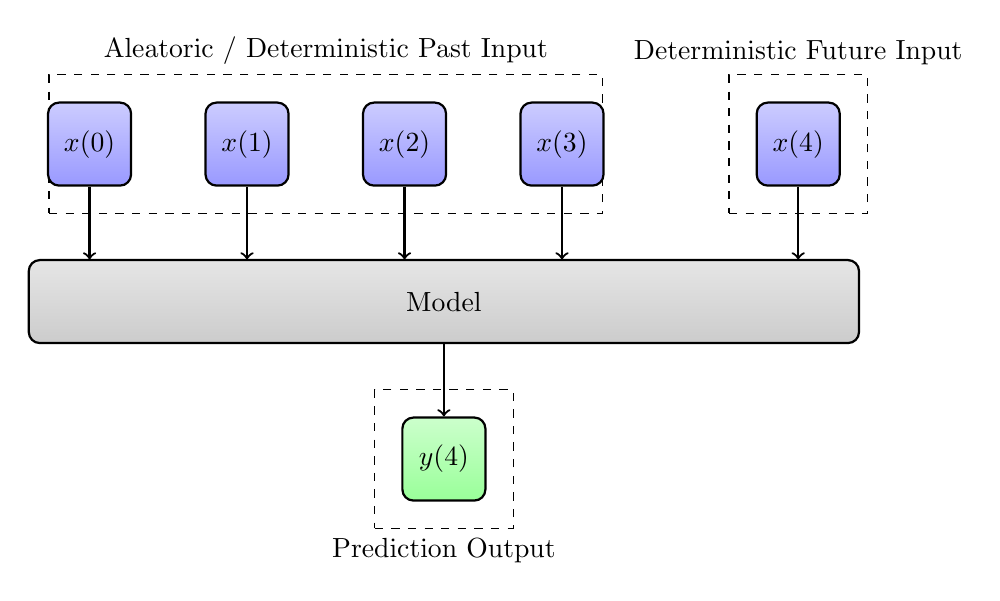
\begin{tikzpicture}[
	input/.style={
		rectangle,
		draw=black,
		thick,
		align=center,
		rounded corners,
		top color=blue!20,
		bottom color=blue!40,
		minimum height=3em,
		minimum width=3em
	},
	model/.style={
		rectangle,
		draw=black,
		thick,
		align=center,
		rounded corners,
		top color=gray!20,
		bottom color=gray!40,
		minimum height=3em,
		minimum width=30em
	},
	hidden/.style={
		rectangle,
		align=center,
		minimum height=3em,
		minimum width=3em
	},
	output/.style={
		rectangle,
		draw=black,
		thick,
		align=center,
		rounded corners,
		top color=green!20,
		bottom color=green!40,
		minimum height=3em,
		minimum width=3em
	},
]

\node[rectangle, dashed, draw=black, align=center, minimum height=5em, minimum width=20em] 
(input) at (0, 2) {};
\node[above] at (input.north) {Aleatoric / Deterministic Past Input};

\node[rectangle, dashed, draw=black, align=center, minimum height=5em, minimum width=5em] 
(input) at (6, 2) {};
\node[above] at (input.north) {Deterministic Future Input};

%\draw[dashed] (-5, 1) rectangle (3, 3);

% Input
\node[input] (in1) at (-3,2) {$x(0)$};
\node[input] (in2) at (-1,2) {$x(1)$};
\node[input] (in3) at (1,2) {$x(2)$};
\node[input] (in4) at (3,2) {$x(3)$};

\node[input] (in5) at (6,2) {$x(4)$};

% Model
\node[model] (mod) at (1.5,0) {Model};
\node[hidden] (mod1) at (-3,0) {};
\node[hidden] (mod2) at (-1,0) {};
\node[hidden] (mod3) at (1,0) {};
\node[hidden] (mod4) at (3,0) {};

\node[hidden] (mod5) at (6,0) {};

\draw[thick,->] (in1.south) -- (mod1.north);
\draw[thick,->] (in2.south) -- (mod2.north);
\draw[thick,->] (in3.south) -- (mod3.north);
\draw[thick,->] (in4.south) -- (mod4.north);

\draw[thick,->] (in5.south) -- (mod5.north);

\node[output] (out1) at (1.5,-2) {$y(4)$};
\draw[thick,->] (mod.south) -- (out1.north);

\node[rectangle, dashed, draw=black, align=center, minimum height=5em, minimum width=5em] 
(output) at (out1.center) {};
\node[below] at (output.south) {Prediction Output};

\end{tikzpicture}
\caption{Prediction example with a \ac{nn} with four time steps in the past and one in the future.}
\label{f:simple_prediction}
\end{figure}

A careful distinction has to be made between the already explained deterministic and aleatoric features. The whole input $\mathbf{x}$ of the \ac{nn} consists of past deterministic and aleatoric features, but also future deterministic features, whose explicit implementation we will see later. \newline
In figure \ref{f:simple_prediction} a simplified example of this whole process is shown. Here the \ac{nn} model takes the last 4 time steps and a deterministic future one as an input to predict the fifth (future) time step.

With this basic concept at hand, we can now go into the next sections and examine the building blocks of \acp{nn}.

	\subsection{Activation Function}
	Before we start with the networks themselves, lets take a look at the mentioned activation function of the nodes. \newline
	Every node has a non-linear activation function, which determines the output based on the input value $z$. The first intentional function - if one takes real neurons as a basis - is the sigmoid function:
	
	\begin{equation}
	S(z) = \frac{1}{1 + e^{-z}}
	\end{equation}
	
	This function saturates with $\lim\limits_{z \to -\infty} \rightarrow 0$ and $\lim\limits_{z \to \infty} \rightarrow 1$. At $z=0$ it has a value of $\frac{1}{2}$ indicating that an negative input makes a neuron activation unlikely and a positive input more likely. Similar to a real neuron that needs a certain signal level to cause an activation.
	
	The other two functions we are going to use are the \ac{relu} and a linear output. 
	
	The way a \ac{relu} works is by cutting off all negative inputs and letting positive ones pass:
	
	\begin{equation}
	g(z) = \max(z, 0)
	\end{equation}
	
	The linear unit doesn't change the output and can be used as the final output for regression problems:
	
	\begin{equation}
	f(z) = z
	\end{equation}

	\subsection{Feed-Forward Layers}
	A Feed-Forward layer is the first type of layers for \acp{nn} \cite[p. 163f]{deep-learning}. It consists of a defined number of (hidden) nodes. These nodes have an output which is described by the activation function shown above. And they have an input that sums up the incoming signals from the previous layer given the weight matrix $\mathbf{W}$ and bias $\mathbf{b}$:
	
	\begin{equation}
	\mathbf{y} = \mathbf{W}\cdot \mathbf{x} + \mathbf{b}
	\end{equation}
	
	Figure \ref{f:fnn_example} shows a \ac{fnn} with 7 input values, 3 hidden layers with different amount of nodes and an output layer with 3 values. It can be seen that every input value $x_n$ is connected with the weight matrix $\mathbf{W}$ and summed up at the input of every node on the following layer. This output is again forwarded to the next layer in the same manner.
	
	\begin{figure}[htb]
	\centering
	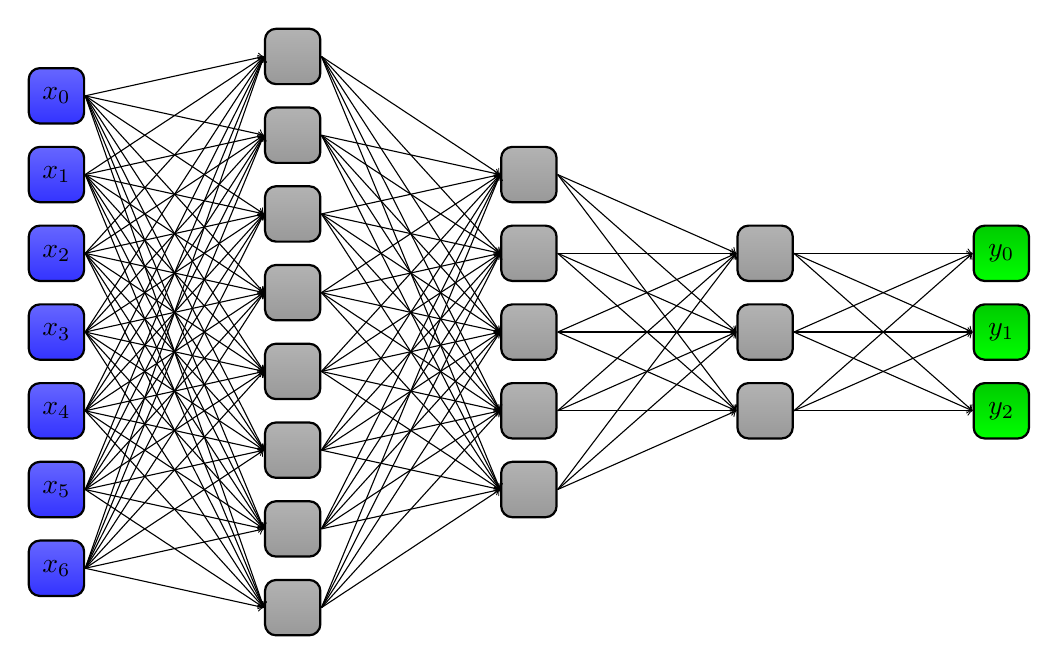
\begin{tikzpicture}[
	input/.style={
		rectangle,
		draw=black,
		thick,
		align=center,
		rounded corners,
		top color=blue!60,
		bottom color=blue!80,
		minimum height=2em,
		minimum width=2em
	},
	neuron/.style={
		rectangle,
		draw=black,
		thick,
		align=center,
		rounded corners,
		top color=gray!60,
		bottom color=gray!80,
		minimum height=2em,
		minimum width=2em
	},
	output/.style={
		rectangle,
		draw=black,
		thick,
		align=center,
		rounded corners,
		top color=green!80!black,
		bottom color=green!100!black,
		minimum height=2em,
		minimum width=2em
	},
]

\foreach \x in {0, ..., 6}
	\node[input] (in\x) at (-6, -\x+3.5) {$x_\x$};

\foreach \x in {0, ..., 7}
	\node[neuron] (nin1\x) at (-3, -\x+4) {};

\foreach \x in {0, ..., 4}
	\node[neuron] (nin2\x) at (0, -\x+2.5) {};

\foreach \x in {0, ..., 2}
	\node[neuron] (nin3\x) at (3, -\x+1.5) {};

\foreach \x in {0, ..., 2}
	\node[output] (out\x) at (6, -\x+1.5) {$y_\x$};


\foreach \x in {0, ..., 6}
	\foreach \y in {0, ..., 7}
		\draw[->] (in\x.east) -- (nin1\y.west);

\foreach \x in {0, ..., 7}
	\foreach \y in {0, ..., 4}
		\draw[->] (nin1\x.east) -- (nin2\y.west);

\foreach \x in {0, ..., 4}
	\foreach \y in {0, ..., 2}
		\draw[->] (nin2\x.east) -- (nin3\y.west);

\foreach \x in {0, ..., 2}
	\foreach \y in {0, ..., 2}
		\draw[->] (nin3\x.east) -- (out\y.west);

\end{tikzpicture}

	\caption{\acf{fnn} with 7 input values $\mathbf{x}$, 3 hidden layers with different amount of nodes and 3 final output values $\mathbf{y}$.}
	\label{f:fnn_example}
	\end{figure}
	
	\subsection{Convolution Layers}
	Convolution is a bit more complex and typically used in image recognition (2 dimensional) rather than time-series analysis (1 dimensional) \cite[p. 321f]{deep-learning}. \newline
	In \acp{nn} the convolution works by sliding a window over the input together with a kernel matrix. This kernel matrix is then trained to extract characteristic features from the data. Usually one starts in the first convolution layer with rough features like edge and shape detection and narrows these down in later layers to more specific features like different objects or parts of the object to be classified.
	
	Figure \ref{f:cnn_example} shows the idea of a convolution layer to extract information or parts from the input data. To refine and specify the features, multiple convolution layers with different input and kernel sizes can be stacked.

	\begin{figure}[htb]
	\centering
	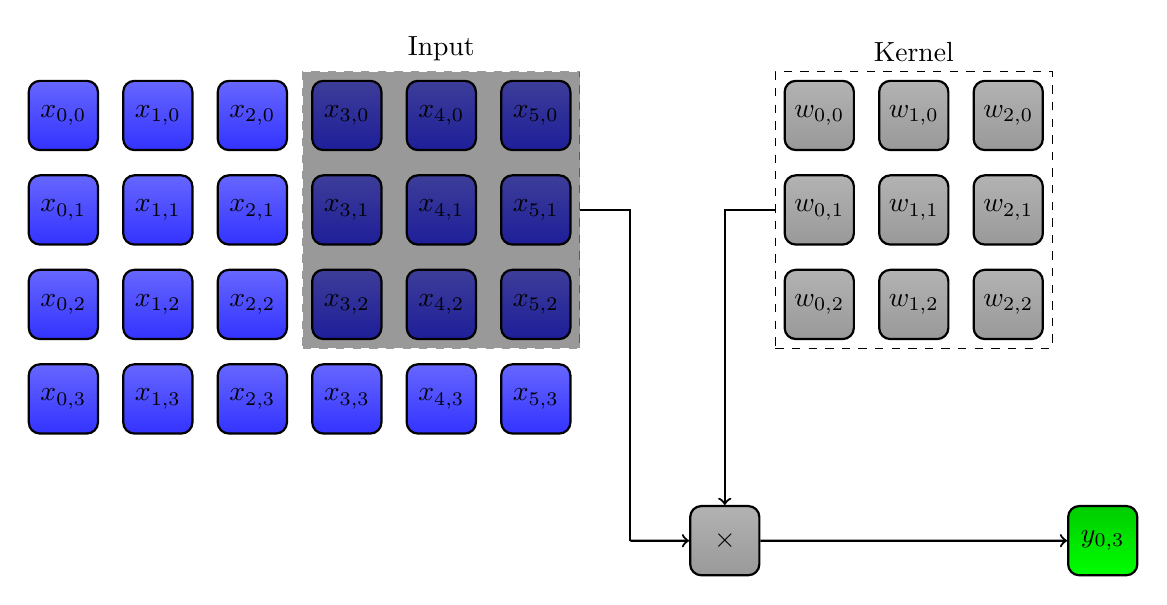
\begin{tikzpicture}[
	input/.style={
		rectangle,
		draw=black,
		thick,
		align=center,
		rounded corners,
		top color=blue!60,
		bottom color=blue!80,
		minimum height=2.5em,
		minimum width=2.5em
	},
	neuron/.style={
		rectangle,
		draw=black,
		thick,
		align=center,
		rounded corners,
		top color=gray!60,
		bottom color=gray!80,
		minimum height=2.5em,
		minimum width=2.5em
	},
	output/.style={
		rectangle,
		draw=black,
		thick,
		align=center,
		rounded corners,
		top color=green!80!black,
		bottom color=green!100!black,
		minimum height=2.5em,
		minimum width=2.5em
	},
	scale=1.2,
]

% Input
\foreach \x in {0, ..., 5}
	\foreach \y in {0, ..., 3}
		\node[input] (in\x\y) at (\x-7, -\y+2) {$x_{\x,\y}$};

\node[rectangle, opacity=0.4,fill=black, dashed, draw=black, align=center, minimum height=10em, minimum width=10em] 
(input) at (in41.center) {};
\node[above] at (input.north) {Input};

% Kernel
\foreach \x in {0, ..., 2}
	\foreach \y in {0, ..., 2}
		\node[neuron] (nin\x\y) at (\x+1, -\y+2) {$w_{\x,\y}$};
 
\node[rectangle, dashed, draw=black, align=center, minimum height=10em, minimum width=10em] 
(kernel) at (nin11) {};
\node[above] at (kernel.north) {Kernel};

\node[neuron] (act) at (0,-2.5) {$\times$};
\node[] (acts) at (-1,-2.5) {};

\node[output] (out) at (4,-2.5) {$y_{0,3}$};

\draw[thick,-, to path={-| (\tikztotarget)}] (input) edge (acts.center);
\draw[thick,->] (acts.center) -- (act);
\draw[thick,->, to path={-| (\tikztotarget)}] (kernel) edge (act);
\draw[thick,->] (act) -- (out);

\end{tikzpicture}

	\caption{\acf{cnn} with input selection on the left and kernel matrix for feature detection on the right.}
	\label{f:cnn_example}
	\end{figure}
	
	\subsection{Long Short-Term Memory}
	The last layer to examine is the \ac{lstm}, belonging to the group of recurrent layers \cite[p. 363f]{deep-learning} \cite{lstm}. \newline
	Recurrent layers or models have - as the name implies - a feedback from their output to their input, making them sensitive to previous (past) input. This is useful within text and speech recognition where the context of past input also matters and not just the current context. In more general terms, \acp{lstm} are useful for sequential inputs, just like time-series data.
	
	Recurrent layers themselves don't bear much problems per se, but stacked in a deep network the back-propagated learning gradient might cause issues by vanishing, exploding or oscillating during the training phase. As a result we will use specifically \ac{lstm} layers, which haven been designed avoid the problem of stacking multiple layers \cite{lstm}.
	
	%Explain LSTM
	In figure \ref{f:lstm_module} the block diagram of an \ac{lstm} cell is shown. \acp{lstm} are nodes which include various gates to mimic a short as well as a long term memory and to avoid the mentioned propagation problems in conventional recurrent units. These gates can specifically \enquote{open} and \enquote{close} to guide information flow and let the model remember and forget information. This helps in understanding the context within the history of a dataset.

	%LSTM figure
	\begin{figure}[htb]
	\centering
	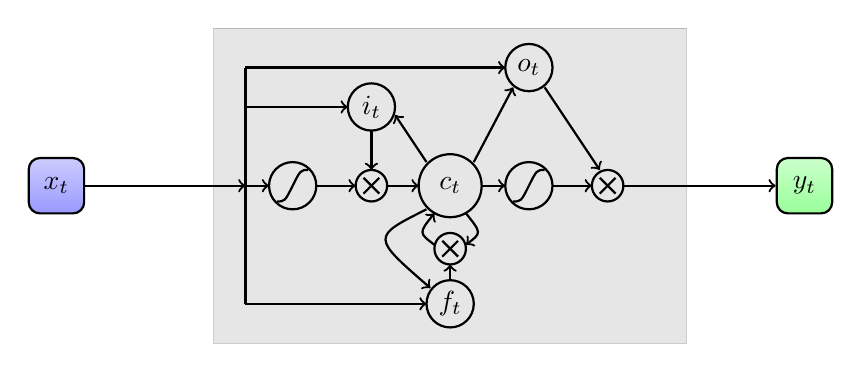
\begin{tikzpicture}[
	input/.style={
		rectangle,
		draw=black,
		thick,
		align=center,
		rounded corners,
		top color=blue!20,
		bottom color=blue!40,
		minimum height=2em,
		minimum width=2em
	},
	neuron/.style={
		rectangle,
		draw=black,
		thick,
		align=center,
		rounded corners,
		top color=gray!20,
		bottom color=gray!40,
		minimum height=2em,
		minimum width=2em
	},
	output/.style={
		rectangle,
		draw=black,
		thick,
		align=center,
		rounded corners,
		top color=green!20,
		bottom color=green!40,
		minimum height=2em,
		minimum width=2em
	},
]


%% Outer box %%
\draw[fill=gray, opacity=0.2] (0,0) rectangle (6,4);

%% Connection arrows %%
% left to right %
%\draw[->, thick] (-0.5, 2) -- (0.4, 2) node[pos=0, above] {$x_t$};
\node[input] (in) at (-2,2) {$x_t$};
\draw[->, thick] (in) -- (0.4, 2);
\draw[->, thick] (0.4, 2) -- (0.7, 2);

\draw[->, thick] (1.3, 2) -- (1.8, 2);
\draw[->, thick] (2.2, 2) -- (2.6, 2);

\draw[->, thick] (3.4, 2) -- (3.7, 2);
\draw[->, thick] (4.3, 2) -- (4.8, 2);

\node[output] (out) at (7.5,2) {$y_t$};
\draw[->, thick] (5.2, 2) -- (out);

% interconnection %
\draw[thick] (0.4, 3.5) -- (0.4, 0.5);
\draw[thick,->] (0.4, 3.5) -- (3.7, 3.5);
\draw[thick,->] (0.4, 0.5) -- (2.7, 0.5);
\draw[thick,->] (0.4, 3) -- (1.7, 3);

\draw[thick,->] (2, 2.7) -- (2, 2.2);
\draw[thick,->] (2.7, 2.3) -- (2.3, 2.9);
\draw[thick,->] (3.3, 2.3) -- (3.8, 3.25);

\draw[thick,->] (4.2, 3.25) -- (4.9, 2.2);

\draw[thick,->] (3, 0.8) -- (3, 1);

\draw[thick,->] (2.7, 1.7) .. controls (2, 1.35) .. (2.75, 0.7);

\draw[thick,->] (2.8, 1.25) .. controls (2.6, 1.4) .. (2.8, 1.65);
\draw[thick,->] (3.2, 1.65) .. controls (3.4, 1.4) .. (3.2, 1.25);

%% Nodes %%
% Sigmoid left %
\draw[thick] (1, 2) circle (0.3);
\draw[thick] (0.8, 1.8) .. controls (0.9, 1.8) .. (1, 2);
\draw[thick] (1, 2) .. controls (1.1, 2.2) .. (1.2, 2.2);

% Multiplication left %
\draw[thick] (2, 2) circle (0.2);
\draw[thick] (1.9, 1.9) -- (2.1, 2.1);
\draw[thick] (2.1, 1.9) -- (1.9, 2.1);

\draw[thick] (3,2) circle(0.4) node {$c_t$};

% Sigmoid right %
\draw[thick] (4, 2) circle (0.3);
\draw[thick] (3.8, 1.8) .. controls (3.9, 1.8) .. (4, 2);
\draw[thick] (4, 2) .. controls (4.1, 2.2) .. (4.2, 2.2);

% Multiplication right %
\draw[thick] (5, 2) circle (0.2);
\draw[thick] (4.9, 1.9) -- (5.1, 2.1);
\draw[thick] (5.1, 1.9) -- (4.9, 2.1);

% input gate %
\draw[thick] (2, 3) circle (0.3) node {$i_t$};

% output gate %
\draw[thick] (4, 3.5) circle (0.3) node {$o_t$};

% forget gate %
\draw[thick] (3, 0.5) circle (0.3) node {$f_t$};
\draw[thick] (3, 1.2) circle (0.2);
\draw[thick] (2.9, 1.1) -- (3.1, 1.3);
\draw[thick] (3.1, 1.1) -- (2.9, 1.3);


\end{tikzpicture}

	\caption{Structure of an \ac{lstm} module. The data $\mathbf{x}_t$ propagates through activation functions (S-circle), is convoluted (X-circle) and gets offset against the internal gates ($i_t$, $o_t$ and $f_t$) to the output $\mathbf{h}_t$.}
	\label{f:lstm_module}
	\end{figure}

	In figure \ref{f:lstm_prediction} the flow of a primitive recurrent model is shown. In contrast to the previous flow we have seen, we do not just have one model block to feed our data in to get our result. In every step we feed a datapoint and transform it trough multiple time steps to finally reach the prediction at $t_N+1$.
	
	\begin{figure}[htb]
	\centering
	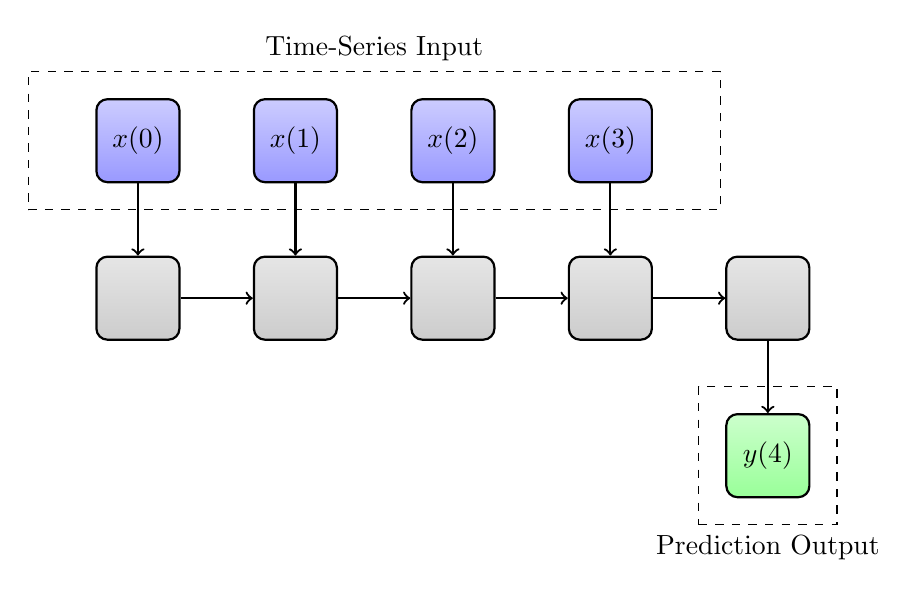
\begin{tikzpicture}[
	input/.style={
		rectangle,
		draw=black,
		thick,
		align=center,
		rounded corners,
		top color=blue!20,
		bottom color=blue!40,
		minimum height=3em,
		minimum width=3em
	},
	neuron/.style={
		rectangle,
		draw=black,
		thick,
		align=center,
		rounded corners,
		top color=gray!20,
		bottom color=gray!40,
		minimum height=3em,
		minimum width=3em
	},
	output/.style={
		rectangle,
		draw=black,
		thick,
		align=center,
		rounded corners,
		top color=green!20,
		bottom color=green!40,
		minimum height=3em,
		minimum width=3em
	},
]

\node[rectangle, dashed, draw=black, align=center, minimum height=5em, minimum width=25em] 
(input) at (-1, 2) {};
\node[above] at (input.north) {Time-Series Input};

%\draw[dashed] (-5, 1) rectangle (3, 3);

\node[input] (in1) at (-4,2) {$x(0)$};
\node[input] (in2) at (-2,2) {$x(1)$};
\node[input] (in3) at (0,2) {$x(2)$};
\node[input] (in4) at (2,2) {$x(3)$};

\node[neuron] (nin1) at (-4,0) {};
\node[neuron] (nin2) at (-2,0) {};
\node[neuron] (nin3) at (0,0) {};
\node[neuron] (nin4) at (2,0) {};

\draw[thick,->] (in1.south) -- (nin1.north);
\draw[thick,->] (in2.south) -- (nin2.north);
\draw[thick,->] (in3.south) -- (nin3.north);
\draw[thick,->] (in4.south) -- (nin4.north);

\draw[thick,->] (nin1.east) -- (nin2.west);
\draw[thick,->] (nin2.east) -- (nin3.west);
\draw[thick,->] (nin3.east) -- (nin4.west);

\node[neuron] (nout1) at (4,0) {};
\draw[thick,->] (nin4.east) -- (nout1.west);

\node[output] (out1) at (4,-2) {$y(4)$};
\draw[thick,->] (nout1.south) -- (out1.north);

\node[rectangle, dashed, draw=black, align=center, minimum height=5em, minimum width=5em] 
(output) at (4, -2) {};
\node[below] at (output.south) {Prediction Output};

\end{tikzpicture}
	\caption{Prediction example with \acfp{lstm}}
	\label{f:lstm_prediction}
	\end{figure}
		
	In the figure \ref{f:rnn_example} below a recurrent network with two hidden layers is shown. With the multiple hidden \enquote{past} layers the idea of a history in the \ac{lstm} cells becomes clear.

	\begin{figure}[htb]
	\centering
	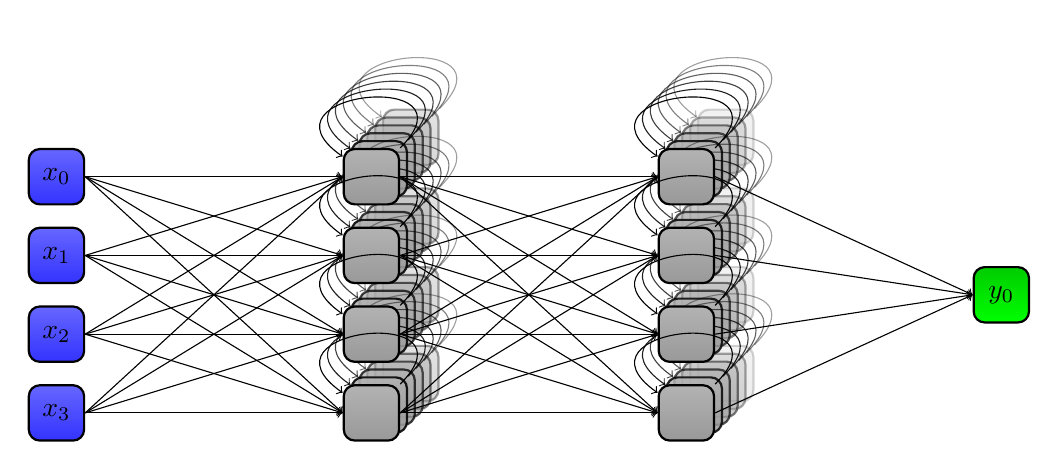
\begin{tikzpicture}[
	input/.style={
		rectangle,
		draw=black,
		thick,
		align=center,
		rounded corners,
		top color=blue!60,
		bottom color=blue!80,
		minimum height=2em,
		minimum width=2em
	},
	neuron/.style={
		rectangle,
		draw=black,
		thick,
		align=center,
		rounded corners,
		top color=gray!60,
		bottom color=gray!80,
		minimum height=2em,
		minimum width=2em
	},
	output/.style={
		rectangle,
		draw=black,
		thick,
		align=center,
		rounded corners,
		top color=green!80!black,
		bottom color=green!100!black,
		minimum height=2em,
		minimum width=2em
	},
]

% Input
\foreach \x in {0, ..., 3}
	\node[input] (in\x) at (-6, -\x+1.5) {$x_\x$};

% Hidden LSTM 1
\foreach \x in {0, ..., 3}
	\foreach \y in {5, ..., 1}
		\node[neuron,opacity=1-\y/8] (nin1h\x\y) at (-2+\y/10, \x-1.5+\y/10) {};

% Connection Hidden LSTM 1
\foreach \x in {0, ..., 3}
	\foreach \y in {5, ..., 1}
		\draw[->,opacity=1-\y/8] (nin1h\x\y) to [out=45,in=145,loop,looseness=5] (nin1h\x\y);

\foreach \x in {0, ..., 3}
	\node[neuron] (nin1\x) at (-2, -\x+1.5) {};

% Hidden LSTM 2
\foreach \x in {0, ..., 3}
	\foreach \y in {5, ..., 1}
		\node[neuron,opacity=1-\y/6] (nin2h\x\y) at (2+\y/10, \x-1.5+\y/10) {};

% Connection Hidden LSTM 2
\foreach \x in {0, ..., 3}
	\foreach \y in {5, ..., 1}
		\draw[->,opacity=1-\y/8] (nin2h\x\y) to [out=45,in=145,loop,looseness=5] (nin2h\x\y);

\foreach \x in {0, ..., 3}
	\node[neuron] (nin2\x) at (2, \x-1.5) {};

% Output
\node[output] (out) at (6, 0) {$y_0$};

%Connection Input
\foreach \x in {0, ..., 3}
	\foreach \y in {0, ..., 3}
		\draw[->] (in\x.east) -- (nin1\y.west);

% Connection Hidden LSTM 1
\foreach \x in {0, ..., 3}
	\draw[->] (nin1\x) to [out=45,in=145,loop,looseness=5] (nin1\x);

% LSTM 1 to LSTM 2
\foreach \x in {0, ..., 3}
	\foreach \y in {0, ..., 3}
		\draw[->] (nin1\x.east) -- (nin2\y.west);

% Connection Hidden LSTM 2
\foreach \x in {0, ..., 3}
	\draw[->] (nin2\x) to [out=45,in=145,loop,looseness=5] (nin2\x);

% Connection Output
\foreach \x in {0, ..., 3}
	\draw[->] (nin2\x.east) -- (out.west);

\end{tikzpicture}

	\caption{Recurrent network example with 4 inputs and 2 hidden \ac{lstm} cell layers feeding back historical information.}
	\label{f:rnn_example}
	\end{figure}
	
	\textbf{Note:} When we want to use past features together with future features as input, special care has to be taken when feeding this information into a recurrent model. Two branches have to be built in order to guide the information flow before we can combine it to a single prediction.
	
	\subsection{Dropout Layer}
	The dropout layer does nothing, except dropping a certain amount of node outputs on a random basis \cite[p. 251f]{deep-learning}. This might at first seem counter-productive, but it is a important step in regularizing the network and extracting uncertainty information. %Yarin Gal made research regarding uncertainty in \acp{nn} and how to extract it via dropout layers \cite{yarin-dropout} \cite{yarin-dropout}.
	An example regarding uncertainty in \acp{nn} and uncertainty extraction via dropout layers can be found in the research made by Yarin Gal \cite{yarin-dropout} \cite{yarin-thesis}.
	
	To get a rough understanding on how this works, consider the following example. Again we want to classify pictures as containing either dogs or cats. If we put a dropout layer at the end, we can randomly mask certain features that might be needed by the network for its classification task. If the picture has a strong indication that there is a cat present as it can find features like facial proportions, ears, tail, fur and whiskers, then masking a few of these features will not change the class. But if there is only a weak indication, then with masking a few features, the networks output changes drastically implying a high variance and therefore high uncertainty in the output.
	
	\subsection{Lambda Layer}
	Lambda layers are specific to Tensorflow and can be filled with a user defined function. In our case we will use it to learn and output a probability distributions. In order to achieve this we have to go one step further and explicitly use the \enquote{DistributionLambda} from the Tensorflow Probability library. This allows for various distributions and applications. We can simply assume a Gaussian normal distribution and output the mean and standard-deviation for a certain input or we can even generate an ensemble of possible outputs that fits our data with a certain probability.

\section{Baseline Model}
Now that we have everything together for building a \ac{nn}, it is time to prepare a quantitative comparison to measure the networks performance. \newline
To get a baseline model we start with the most primitive idea and see if it fulfils the given criteria and requirements. As we have not seen any periodicity in the data we assume that no specific adaptations have to be made when we choose a certain $\Delta t$ for the future prediction. Secondly, any expert knowledge is kept out of the baseline creation process as our \ac{nn} will have a similar requirement to avoid any bias and to be more universal. And at last, the baseline shall only depend on the current time-window with past and future values of our interest and without any other history or features. Therefore we chose a baseline model, that assumes the future values will be the same as the past seen ones:

\begin{equation}
x(t_N + 24) = x(t_N) + \varepsilon
\end{equation}

whereas $\varepsilon$ is the error and our measurement for the \ac{nn}. If the \ac{nn} is able to generate a result with a smaller $\varepsilon$ than the baseline model, it is considered to be a success.\newline
In table \ref{t:baseline_error} the absolute baseline error $| \varepsilon |$ for the different datasets from our example Rosetta is given. They were collected and averaged over the complete dataset. This will later be used for comparison.

\begin{table}[htb]
\centering
\caption{Baseline model prediction error for the respective Rosetta housekeeping datasets}
\begin{tabular}{lll}
\toprule
Dataset				& $| \varepsilon_{Base} |$ \\ \midrule
Wheel A Friction		& $\num{0.0233}$		\\
Wheel B Friction		& $\num{0.0242}$		\\
Wheel C Friction		& $\num{0.0266}$		\\
Wheel D Friction		& $\num{0.0300}$		\\
Solar Array Voltage	& $\num{0.0065}$		\\
\bottomrule
\end{tabular}
\label{t:baseline_error}
\end{table}
		
\section{Predicting Rosetta Housekeeping Data}
Now that we have have all the building blocks and a baseline for comparison, we can assemble our network and use it on the Rosetta housekeeping data. We want to see if we are able to predict the future values with more accuracy than the baseline and check if the uncertainty fits the data distribution. A special look will be taken at the data of reaction wheel B as this failed in 2008. There we will try to predict the friction value which the engineers in \cite{rosetta-maintenance} identified as anomalous.

In the next sections we will first build a \ac{nn} model for our predictions. To understand all the necessary steps, we look at how the uncertainty output is created, which optimizer is used, what hyperparameters are chosen and how the data and features are set up. Finally the source code of the model itself is given and described briefly. \newline
After all is prepared, the network can be trained and compared to the baseline established in the section above.

	\subsection{Neural Network Model}
	Now for hands-on praxis, we will develop our \ac{nn} model in the following sections. \newline
	As an underlying framework, we use the previously described Tensorflow with Tensorflow Probabilities for Python \cite{tf-web}. In this framework we will stack together the layers we discussed in chapter \ref{c:nn-blocks} together with a probability output layer. Then we will set our hyperparameters and optimizer. At the end, the source code for a generic model is presented.	
	
		\subsubsection{Uncertainty}
		The uncertainty of a prediction is embedded in the Tensorflow Probabilities. It will be the last layer of our network outputting a probability distribution as a prediction. 
		
		To understand this kind of output, we will take a look at noisy (normally distributed) dataset in figure \ref{f:tfp_example_1} as an example\footnote{Taken from \cite{tf-prop-example}}. Here we want to apply our regression analysis. The first stage is to make a linear interpolation fitting the points with the least mean squared error (see code \ref{p:tfp_example_1}). \newline
		Now we introduce probabilities. For that we will change the first layer and add prior assumptions to our data. The model contains a distribution as an output and will not only give the most probable linear interpolation, but also the variance estimated from the data. This we can put to use and actually produce an ensemble of different curves that would fit the dataset with a certain probability, as it can be seen in figure \ref{f:tfp_example_2}. \newline
		Finally, we can not only estimate mean and variance, but actually the kind of distribution the data represents. If we add that estimation to the code \ref{p:tfp_example_3} we will get the result in figure \ref{f:tfp_example_3}, where we now can see, that the dataset represents most likely a noisy sine with increasing amplitude.
		
		\begin{figure}[htb]
		\centering
		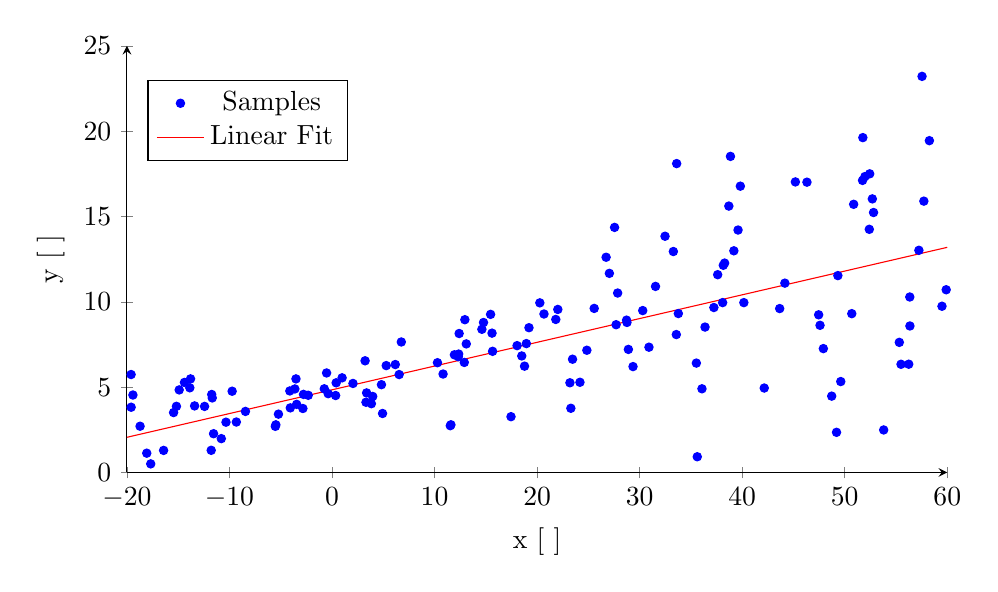
\begin{tikzpicture}
	\begin{axis}[
		xlabel={x [ ]},
		ylabel={y [ ]},
		height=7cm,
		width=12cm,
		ymin=0, ymax=25,
		axis x line=bottom,
		axis y line=left,
		legend style={at={(axis cs:-18,23)},anchor=north west}
]
	\addplot[only marks, mark size=1.5pt, color=blue, mark=*] plot coordinates {
		(-10.795634688817684, 1.9829061646124744)
		(28.725323142358512, 8.924186913651395)
		(-9.328722865120938, 2.955337623514433)
		(-0.7528304027720978, 4.901770489885887)
		(6.171124464891182, 6.323897217895851)
		(48.73099927588781, 4.4722330939169295)
		(33.28721704784206, 12.946408488661683)
		(23.2929769826723, 3.7609858008274655)
		(-17.67889404605117, 0.502763471069544)
		(38.69986370242263, 15.609062872915612)
		(11.596001474480468, 2.793908600708612)
		(44.16376949029332, 11.093302037978546)
		(0.3536900687903426, 4.507914077058895)
		(-15.449205067907856, 3.509580365638704)
		(49.331891271936016, 11.53538889896722)
		(-2.317680329250294, 4.522451274117105)
		(12.399155843780775, 8.141812027689982)
		(5.287717681456698, 6.26145650784877)
		(-13.86698400028422, 4.960066195837447)
		(47.45797553837636, 9.238163343301192)
		(47.91513181958892, 7.257348088523997)
		(57.71720731483103, 15.898294392366129)
		(10.83015315161105, 5.767894815676739)
		(56.35905000869322, 8.582923204158066)
		(15.660668867177506, 7.098244654937592)
		(33.57797213774462, 8.080144784396026)
		(-13.399996024227567, 3.9000360766265465)
		(51.76788639852275, 19.620089149251385)
		(3.840280055101015, 4.029361546231701)
		(0.9843858077105168, 5.544947118195031)
		(-19.589636074843444, 3.8221093951008576)
		(23.45620122243248, 6.635477691030698)
		(18.047709360580257, 7.431803030385503)
		(30.90989420572181, 7.339960162078889)
		(58.25633072656049, 19.44215404359411)
		(52.69302062648703, 16.030718371820793)
		(52.81224606241253, 15.231435143810064)
		(22.020453688571635, 9.551957694763209)
		(-11.678484011618968, 4.367712354781274)
		(-5.526832379367921, 2.704002481738616)
		(56.24321767893933, 6.343101962486358)
		(12.95623867090869, 8.951447105839712)
		(49.20136964857454, 2.351872616453877)
		(33.77418235809409, 9.312102867360167)
		(30.302863670572897, 9.48553745520231)
		(2.044702131916168, 5.214822459385231)
		(51.73978157926901, 17.11378049067176)
		(-3.4486902925307845, 3.991636410596644)
		(12.352419446032606, 6.937444377172751)
		(59.48579939152828, 9.73990268714271)
		(38.85816652056966, 18.520788609638885)
		(15.604912999174616, 8.163544079564328)
		(24.8530535554988, 7.161329692460491)
		(12.90043912693082, 6.447583532400695)
		(38.15903935743908, 12.13998709825581)
		(11.935750872325984, 6.894308731525425)
		(33.611613176190545, 18.09846316361692)
		(36.37724863044332, 8.519610782799358)
		(28.76478970072366, 8.790719804927814)
		(23.202757134532483, 5.255037853885915)
		(-3.5134519269358577, 5.482653549195127)
		(-4.0670818701838485, 3.784428534828735)
		(43.65910918528353, 9.603529211466006)
		(3.226622221660527, 6.543141091320835)
		(32.477026225908304, 13.84158879347751)
		(3.969342064561985, 4.4532559061246735)
		(-8.441729726173701, 3.577359912358882)
		(12.31653335843756, 6.780541146566437)
		(4.821562147567178, 5.143448670851623)
		(-0.5281586975230184, 5.830027796384844)
		(27.048323412670086, 11.666582515867482)
		(-0.3725397629312184, 4.617149344641111)
		(39.82164894342905, 16.775239991583117)
		(37.61173182833783, 11.588507637149362)
		(35.62086935640743, 0.9205110420501752)
		(-11.780577714143066, 1.2983066278421092)
		(55.49139425474328, 6.338878598423139)
		(20.267170631422545, 9.938615559837364)
		(51.97388954939302, 17.33777298684131)
		(-4.113609245094887, 4.776478505193331)
		(27.555934945474466, 14.359860846913378)
		(57.232686534181056, 13.017286820304465)
		(59.89585967173496, 10.705821666779132)
		(-18.06651000155643, 1.1294972752086043)
		(18.50426667642533, 6.826783755269135)
		(3.313815173888635, 4.113749206259239)
		(-14.902354534614837, 4.83701675007238)
		(25.56995191544472, 9.612830115907272)
		(-19.59333722406288, 5.738436395310126)
		(28.90220717360173, 7.2105146904691075)
		(49.61451816276716, 5.327054373305876)
		(50.68811719791114, 9.305241152060212)
		(56.34555865568306, 10.281412429798754)
		(39.18910558427793, 12.987985028319274)
		(-5.222963396072897, 3.41640514785584)
		(14.774265686944418, 8.786441224548218)
		(50.87195964382987, 15.713074186954168)
		(0.4037024267837168, 5.2535501587171485)
		(15.465015578318727, 9.2632141183608)
		(29.35495806567161, 6.203845899484306)
		(-11.731799129747644, 4.568918535753642)
		(19.208772885525, 8.48244395832387)
		(-16.42364780514025, 1.2924178264361914)
		(4.93019754473206, 3.455584633987355)
		(40.163174909282006, 9.95167283183368)
		(37.239926922245175, 9.664630271743851)
		(55.32433950066536, 7.62351800966176)
		(42.15162933670156, 4.947224154328223)
		(-2.781718801025104, 4.575269058334888)
		(52.39769445066004, 14.247581365412492)
		(24.181131760912287, 5.2841515524643485)
		(47.591831006148496, 8.622768780458518)
		(53.79915870184324, 2.490876607733414)
		(46.316902315131344, 17.009812807658246)
		(11.535839836778106, 2.7398924437038685)
		(27.85505092657013, 10.513850502768712)
		(14.615846365088018, 8.389986165315394)
		(35.531770859756065, 6.4083779853776495)
		(18.77491916829012, 6.228452915938787)
		(-9.73917267391414, 4.759820059299385)
		(31.54963972910509, 10.902514478405172)
		(-3.6235027063475833, 4.893580688364125)
		(39.59657004257837, 14.20529446769158)
		(-11.550623487793388, 2.270140347591962)
		(-19.41524050208602, 4.538316727552468)
		(6.759119324234586, 7.645822334110396)
		(57.54044030648447, 23.209044843123976)
		(36.07805515466435, 4.902524833220188)
		(13.094842778666909, 7.533818477378985)
		(-10.339826358737003, 2.9459063124130958)
		(-15.170916451875708, 3.874619764914822)
		(38.09693390086201, 9.952902749194662)
		(52.43607874507789, 17.49917530926083)
		(-18.717926565430485, 2.7085258646006727)
		(26.731266457086942, 12.610406057590884)
		(38.28832401668412, 12.268723750110976)
		(3.3758035420806536, 4.661967044701783)
		(21.82380930617949, 8.966169871794405)
		(45.18815090004941, 17.02456636469129)
		(27.706158414149257, 8.65709761325555)
		(10.284427156125588, 6.431136055867023)
		(-13.795375560402324, 5.483836106667359)
		(18.952494098566905, 7.551320729556901)
		(17.455512485594014, 3.2685035428718257)
		(-5.477219461651952, 2.790732378027741)
		(-14.389125242941024, 5.275462205559022)
		(20.672074571712518, 9.285062286784688)
		(6.548138786502243, 5.736719752321169)
		(-2.8401743722468424, 3.7478905091463366)
		(-12.4274484628451, 3.871030685943469)
	};
	\addlegendentry{Samples}
	\addplot[mark size=2.5pt, color=red] plot coordinates {
		(-20.0, 2.060235)
		(60.0, 13.191476)
	};
	\addlegendentry{Linear Fit}
	\end{axis}
\end{tikzpicture}

		\caption{Stochastic randomly distributed data with a linear fit}
		\label{f:tfp_example_1}
		\end{figure}

		\begin{lstlisting}[caption={Linear Fit}, language=python, label={p:tfp_example_1}]
model = tf.keras.Sequential([
  tf.keras.layers.Dense(1),
  tfp.layers.DistributionLambda(
    lambda t: tfd.Normal(loc=t, scale=1))])		
		\end{lstlisting}
		
		\begin{figure}[htb]
		\centering
		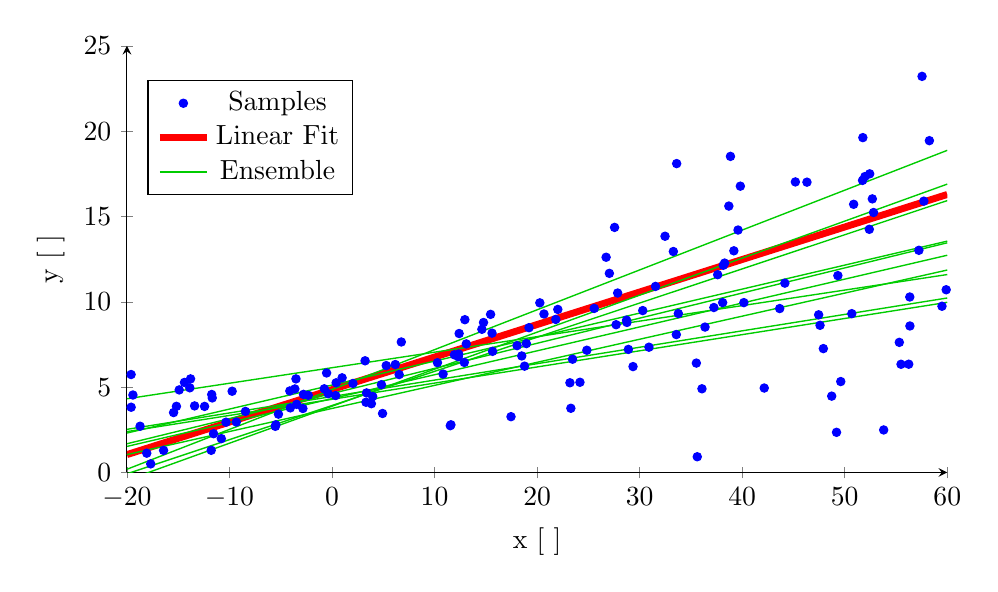
\begin{tikzpicture}[
	ens/.style={
		line width=0.5pt, 
		color=green!80!black,	
	},
]
	\begin{axis}[
		xlabel={x [ ]},
		ylabel={y [ ]},
		height=7cm,
		width=12cm,
		ymin=0, ymax=25,
		axis x line=bottom,
		axis y line=left,
		legend style={at={(axis cs:-18,23)},anchor=north west}
]
	\addplot[only marks, mark size=1.5pt, color=blue, mark=*] plot coordinates {
		(-10.7956346888177, 1.98290616461247)
		(28.7253231423585, 8.9241869136514)
		(-9.32872286512094, 2.95533762351443)
		(-0.752830402772098, 4.90177048988589)
		(6.17112446489118, 6.32389721789585)
		(48.7309992758878, 4.47223309391693)
		(33.2872170478421, 12.9464084886617)
		(23.2929769826723, 3.76098580082747)
		(-17.6788940460512, 0.502763471069544)
		(38.6998637024226, 15.6090628729156)
		(11.5960014744805, 2.79390860070861)
		(44.1637694902933, 11.0933020379785)
		(0.353690068790343, 4.5079140770589)
		(-15.4492050679079, 3.5095803656387)
		(49.331891271936, 11.5353888989672)
		(-2.31768032925029, 4.52245127411711)
		(12.3991558437808, 8.14181202768998)
		(5.2877176814567, 6.26145650784877)
		(-13.8669840002842, 4.96006619583745)
		(47.4579755383764, 9.23816334330119)
		(47.9151318195889, 7.257348088524)
		(57.717207314831, 15.8982943923661)
		(10.8301531516111, 5.76789481567674)
		(56.3590500086932, 8.58292320415807)
		(15.6606688671775, 7.09824465493759)
		(33.5779721377446, 8.08014478439603)
		(-13.3999960242276, 3.90003607662655)
		(51.7678863985227, 19.6200891492514)
		(3.84028005510102, 4.0293615462317)
		(0.984385807710517, 5.54494711819503)
		(-19.5896360748434, 3.82210939510086)
		(23.4562012224325, 6.6354776910307)
		(18.0477093605803, 7.4318030303855)
		(30.9098942057218, 7.33996016207889)
		(58.2563307265605, 19.4421540435941)
		(52.693020626487, 16.0307183718208)
		(52.8122460624125, 15.2314351438101)
		(22.0204536885716, 9.55195769476321)
		(-11.678484011619, 4.36771235478127)
		(-5.52683237936792, 2.70400248173862)
		(56.2432176789393, 6.34310196248636)
		(12.9562386709087, 8.95144710583971)
		(49.2013696485745, 2.35187261645388)
		(33.7741823580941, 9.31210286736017)
		(30.3028636705729, 9.48553745520231)
		(2.04470213191617, 5.21482245938523)
		(51.739781579269, 17.1137804906718)
		(-3.44869029253078, 3.99163641059664)
		(12.3524194460326, 6.93744437717275)
		(59.4857993915283, 9.73990268714271)
		(38.8581665205697, 18.5207886096389)
		(15.6049129991746, 8.16354407956433)
		(24.8530535554988, 7.16132969246049)
		(12.9004391269308, 6.4475835324007)
		(38.1590393574391, 12.1399870982558)
		(11.935750872326, 6.89430873152543)
		(33.6116131761905, 18.0984631636169)
		(36.3772486304433, 8.51961078279936)
		(28.7647897007237, 8.79071980492781)
		(23.2027571345325, 5.25503785388591)
		(-3.51345192693586, 5.48265354919513)
		(-4.06708187018385, 3.78442853482874)
		(43.6591091852835, 9.60352921146601)
		(3.22662222166053, 6.54314109132084)
		(32.4770262259083, 13.8415887934775)
		(3.96934206456199, 4.45325590612467)
		(-8.4417297261737, 3.57735991235888)
		(12.3165333584376, 6.78054114656644)
		(4.82156214756718, 5.14344867085162)
		(-0.528158697523018, 5.83002779638484)
		(27.0483234126701, 11.6665825158675)
		(-0.372539762931218, 4.61714934464111)
		(39.821648943429, 16.7752399915831)
		(37.6117318283378, 11.5885076371494)
		(35.6208693564074, 0.920511042050175)
		(-11.7805777141431, 1.29830662784211)
		(55.4913942547433, 6.33887859842314)
		(20.2671706314225, 9.93861555983736)
		(51.973889549393, 17.3377729868413)
		(-4.11360924509489, 4.77647850519333)
		(27.5559349454745, 14.3598608469134)
		(57.2326865341811, 13.0172868203045)
		(59.895859671735, 10.7058216667791)
		(-18.0665100015564, 1.1294972752086)
		(18.5042666764253, 6.82678375526914)
		(3.31381517388863, 4.11374920625924)
		(-14.9023545346148, 4.83701675007238)
		(25.5699519154447, 9.61283011590727)
		(-19.5933372240629, 5.73843639531013)
		(28.9022071736017, 7.21051469046911)
		(49.6145181627672, 5.32705437330588)
		(50.6881171979111, 9.30524115206021)
		(56.3455586556831, 10.2814124297988)
		(39.1891055842779, 12.9879850283193)
		(-5.2229633960729, 3.41640514785584)
		(14.7742656869444, 8.78644122454822)
		(50.8719596438299, 15.7130741869542)
		(0.403702426783717, 5.25355015871715)
		(15.4650155783187, 9.2632141183608)
		(29.3549580656716, 6.20384589948431)
		(-11.7317991297476, 4.56891853575364)
		(19.208772885525, 8.48244395832387)
		(-16.4236478051403, 1.29241782643619)
		(4.93019754473206, 3.45558463398735)
		(40.163174909282, 9.95167283183368)
		(37.2399269222452, 9.66463027174385)
		(55.3243395006654, 7.62351800966176)
		(42.1516293367016, 4.94722415432822)
		(-2.7817188010251, 4.57526905833489)
		(52.39769445066, 14.2475813654125)
		(24.1811317609123, 5.28415155246435)
		(47.5918310061485, 8.62276878045852)
		(53.7991587018432, 2.49087660773341)
		(46.3169023151314, 17.0098128076582)
		(11.5358398367781, 2.73989244370387)
		(27.8550509265701, 10.5138505027687)
		(14.615846365088, 8.38998616531539)
		(35.5317708597561, 6.40837798537765)
		(18.7749191682901, 6.22845291593879)
		(-9.73917267391414, 4.75982005929939)
		(31.5496397291051, 10.9025144784052)
		(-3.62350270634758, 4.89358068836413)
		(39.5965700425784, 14.2052944676916)
		(-11.5506234877934, 2.27014034759196)
		(-19.415240502086, 4.53831672755247)
		(6.75911932423459, 7.6458223341104)
		(57.5404403064845, 23.209044843124)
		(36.0780551546643, 4.90252483322019)
		(13.0948427786669, 7.53381847737899)
		(-10.339826358737, 2.9459063124131)
		(-15.1709164518757, 3.87461976491482)
		(38.096933900862, 9.95290274919466)
		(52.4360787450779, 17.4991753092608)
		(-18.7179265654305, 2.70852586460067)
		(26.7312664570869, 12.6104060575909)
		(38.2883240166841, 12.268723750111)
		(3.37580354208065, 4.66196704470178)
		(21.8238093061795, 8.9661698717944)
		(45.1881509000494, 17.0245663646913)
		(27.7061584141493, 8.65709761325555)
		(10.2844271561256, 6.43113605586702)
		(-13.7953755604023, 5.48383610666736)
		(18.9524940985669, 7.5513207295569)
		(17.455512485594, 3.26850354287183)
		(-5.47721946165195, 2.79073237802774)
		(-14.389125242941, 5.27546220555902)
		(20.6720745717125, 9.28506228678469)
		(6.54813878650224, 5.73671975232117)
		(-2.84017437224684, 3.74789050914634)
		(-12.4274484628451, 3.87103068594347)
	};
	\addlegendentry{Samples}
	\addplot[line width=2.5pt, color=red] plot coordinates {
		(-20, 1.0460736)
		(60, 16.288374)
	};
	\addlegendentry{Linear Fit}
	\addplot[ens] plot coordinates {
		(-20.0, 0.18711138)
		(60.0, 18.874634)
	};
	\addlegendentry{Ensemble}
	\addplot[ens] plot coordinates {
		(-20.0, -0.45565867)
		(60.0, 16.895638)
	};
	\addplot[ens] plot coordinates {
		(-20.0, 2.5253172)
		(60.0, 10.223032)
	};
	\addplot[ens] plot coordinates {
		(-20.0, 1.6817)
		(60.0, 13.4572525)
	};
	\addplot[ens] plot coordinates {
		(-20.0, 1.047251)
		(60.0, 11.861124)
	};
	\addplot[ens] plot coordinates {
		(-20.0, 2.309102)
		(60.0, 13.554658)
	};
	\addplot[ens] plot coordinates {
		(-20.0, 1.5259745)
		(60.0, 12.727637)
	};
	\addplot[ens] plot coordinates {
		(-20.0, 2.3945184)
		(60.0, 9.969112)
	};
	\addplot[ens] plot coordinates {
		(-20.0, 4.318074)
		(60.0, 11.596326)
	};
	\addplot[ens] plot coordinates {
		(-20.0, -0.07831025)
		(60.0, 15.929726)
	};
	\end{axis}
\end{tikzpicture}

		\caption{Stochastic randomly distributed data with an ensemble of probable linear fits}
		\label{f:tfp_example_2}
		\end{figure}
		
		\begin{figure}[htb]
		\centering
		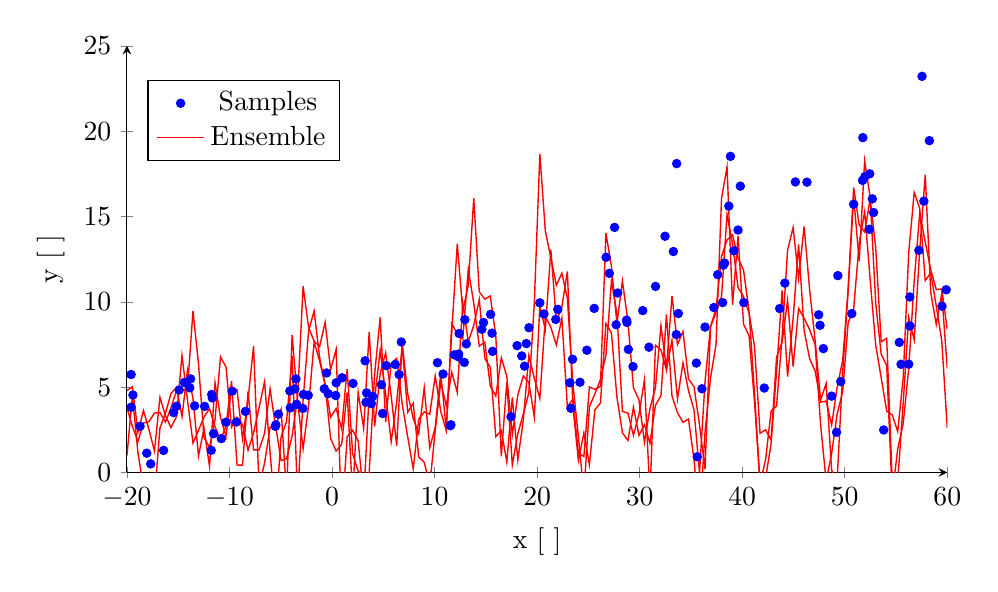
\begin{tikzpicture}[
	ens/.style={
		line width=0.5pt, 
		color=red,	
	},
]
	\begin{axis}[
		xlabel={x [ ]},
		ylabel={y [ ]},
		height=7cm,
		width=12cm,
		ymin=0, ymax=25,
		axis x line=bottom,
		axis y line=left,
		legend style={at={(axis cs:-18,23)},anchor=north west}
]
	\addplot[only marks, mark size=1.5pt, color=blue, mark=*] plot coordinates {
		(-10.795634688817684, 1.9829061646124744)
		(28.725323142358512, 8.924186913651395)
		(-9.328722865120938, 2.955337623514433)
		(-0.7528304027720978, 4.901770489885887)
		(6.171124464891182, 6.323897217895851)
		(48.73099927588781, 4.4722330939169295)
		(33.28721704784206, 12.946408488661683)
		(23.2929769826723, 3.7609858008274655)
		(-17.67889404605117, 0.502763471069544)
		(38.69986370242263, 15.609062872915612)
		(11.596001474480468, 2.793908600708612)
		(44.16376949029332, 11.093302037978546)
		(0.3536900687903426, 4.507914077058895)
		(-15.449205067907856, 3.509580365638704)
		(49.331891271936016, 11.53538889896722)
		(-2.317680329250294, 4.522451274117105)
		(12.399155843780775, 8.141812027689982)
		(5.287717681456698, 6.26145650784877)
		(-13.86698400028422, 4.960066195837447)
		(47.45797553837636, 9.238163343301192)
		(47.91513181958892, 7.257348088523997)
		(57.71720731483103, 15.898294392366129)
		(10.83015315161105, 5.767894815676739)
		(56.35905000869322, 8.582923204158066)
		(15.660668867177506, 7.098244654937592)
		(33.57797213774462, 8.080144784396026)
		(-13.399996024227567, 3.9000360766265465)
		(51.76788639852275, 19.620089149251385)
		(3.840280055101015, 4.029361546231701)
		(0.9843858077105168, 5.544947118195031)
		(-19.589636074843444, 3.8221093951008576)
		(23.45620122243248, 6.635477691030698)
		(18.047709360580257, 7.431803030385503)
		(30.90989420572181, 7.339960162078889)
		(58.25633072656049, 19.44215404359411)
		(52.69302062648703, 16.030718371820793)
		(52.81224606241253, 15.231435143810064)
		(22.020453688571635, 9.551957694763209)
		(-11.678484011618968, 4.367712354781274)
		(-5.526832379367921, 2.704002481738616)
		(56.24321767893933, 6.343101962486358)
		(12.95623867090869, 8.951447105839712)
		(49.20136964857454, 2.351872616453877)
		(33.77418235809409, 9.312102867360167)
		(30.302863670572897, 9.48553745520231)
		(2.044702131916168, 5.214822459385231)
		(51.73978157926901, 17.11378049067176)
		(-3.4486902925307845, 3.991636410596644)
		(12.352419446032606, 6.937444377172751)
		(59.48579939152828, 9.73990268714271)
		(38.85816652056966, 18.520788609638885)
		(15.604912999174616, 8.163544079564328)
		(24.8530535554988, 7.161329692460491)
		(12.90043912693082, 6.447583532400695)
		(38.15903935743908, 12.13998709825581)
		(11.935750872325984, 6.894308731525425)
		(33.611613176190545, 18.09846316361692)
		(36.37724863044332, 8.519610782799358)
		(28.76478970072366, 8.790719804927814)
		(23.202757134532483, 5.255037853885915)
		(-3.5134519269358577, 5.482653549195127)
		(-4.0670818701838485, 3.784428534828735)
		(43.65910918528353, 9.603529211466006)
		(3.226622221660527, 6.543141091320835)
		(32.477026225908304, 13.84158879347751)
		(3.969342064561985, 4.4532559061246735)
		(-8.441729726173701, 3.577359912358882)
		(12.31653335843756, 6.780541146566437)
		(4.821562147567178, 5.143448670851623)
		(-0.5281586975230184, 5.830027796384844)
		(27.048323412670086, 11.666582515867482)
		(-0.3725397629312184, 4.617149344641111)
		(39.82164894342905, 16.775239991583117)
		(37.61173182833783, 11.588507637149362)
		(35.62086935640743, 0.9205110420501752)
		(-11.780577714143066, 1.2983066278421092)
		(55.49139425474328, 6.338878598423139)
		(20.267170631422545, 9.938615559837364)
		(51.97388954939302, 17.33777298684131)
		(-4.113609245094887, 4.776478505193331)
		(27.555934945474466, 14.359860846913378)
		(57.232686534181056, 13.017286820304465)
		(59.89585967173496, 10.705821666779132)
		(-18.06651000155643, 1.1294972752086043)
		(18.50426667642533, 6.826783755269135)
		(3.313815173888635, 4.113749206259239)
		(-14.902354534614837, 4.83701675007238)
		(25.56995191544472, 9.612830115907272)
		(-19.59333722406288, 5.738436395310126)
		(28.90220717360173, 7.2105146904691075)
		(49.61451816276716, 5.327054373305876)
		(50.68811719791114, 9.305241152060212)
		(56.34555865568306, 10.281412429798754)
		(39.18910558427793, 12.987985028319274)
		(-5.222963396072897, 3.41640514785584)
		(14.774265686944418, 8.786441224548218)
		(50.87195964382987, 15.713074186954168)
		(0.4037024267837168, 5.2535501587171485)
		(15.465015578318727, 9.2632141183608)
		(29.35495806567161, 6.203845899484306)
		(-11.731799129747644, 4.568918535753642)
		(19.208772885525, 8.48244395832387)
		(-16.42364780514025, 1.2924178264361914)
		(4.93019754473206, 3.455584633987355)
		(40.163174909282006, 9.95167283183368)
		(37.239926922245175, 9.664630271743851)
		(55.32433950066536, 7.62351800966176)
		(42.15162933670156, 4.947224154328223)
		(-2.781718801025104, 4.575269058334888)
		(52.39769445066004, 14.247581365412492)
		(24.181131760912287, 5.2841515524643485)
		(47.591831006148496, 8.622768780458518)
		(53.79915870184324, 2.490876607733414)
		(46.316902315131344, 17.009812807658246)
		(11.535839836778106, 2.7398924437038685)
		(27.85505092657013, 10.513850502768712)
		(14.615846365088018, 8.389986165315394)
		(35.531770859756065, 6.4083779853776495)
		(18.77491916829012, 6.228452915938787)
		(-9.73917267391414, 4.759820059299385)
		(31.54963972910509, 10.902514478405172)
		(-3.6235027063475833, 4.893580688364125)
		(39.59657004257837, 14.20529446769158)
		(-11.550623487793388, 2.270140347591962)
		(-19.41524050208602, 4.538316727552468)
		(6.759119324234586, 7.645822334110396)
		(57.54044030648447, 23.209044843123976)
		(36.07805515466435, 4.902524833220188)
		(13.094842778666909, 7.533818477378985)
		(-10.339826358737003, 2.9459063124130958)
		(-15.170916451875708, 3.874619764914822)
		(38.09693390086201, 9.952902749194662)
		(52.43607874507789, 17.49917530926083)
		(-18.717926565430485, 2.7085258646006727)
		(26.731266457086942, 12.610406057590884)
		(38.28832401668412, 12.268723750110976)
		(3.3758035420806536, 4.661967044701783)
		(21.82380930617949, 8.966169871794405)
		(45.18815090004941, 17.02456636469129)
		(27.706158414149257, 8.65709761325555)
		(10.284427156125588, 6.431136055867023)
		(-13.795375560402324, 5.483836106667359)
		(18.952494098566905, 7.551320729556901)
		(17.455512485594014, 3.2685035428718257)
		(-5.477219461651952, 2.790732378027741)
		(-14.389125242941024, 5.275462205559022)
		(20.672074571712518, 9.285062286784688)
		(6.548138786502243, 5.736719752321169)
		(-2.8401743722468424, 3.7478905091463366)
		(-12.4274484628451, 3.871030685943469)
	};
	\addlegendentry{Samples}
	\addplot[ens] plot coordinates {
		(-20.0, 0.987559537050878)
		(-19.463087, 4.489530450288576)
		(-18.926174, 1.1667457094410856)
		(-18.389261, -0.8950225640420233)
		(-17.852348, -1.5050971284336372)
		(-17.315435, -1.4420030957674186)
		(-16.778524, 2.604228577934319)
		(-16.241611, 3.469191300953715)
		(-15.704698, 4.631203700765719)
		(-15.167786, 4.979930568688454)
		(-14.630873, 3.2760359277507205)
		(-14.09396, 5.991695652426456)
		(-13.557047, 4.319719602323335)
		(-13.020134, 0.974070398770774)
		(-12.483221, 2.5912032080413208)
		(-11.946309, 0.3580804828325443)
		(-11.409396, 5.261672963603872)
		(-10.872483, 3.217385709314435)
		(-10.33557, 2.0976224282575693)
		(-9.798657, 4.966536146420354)
		(-9.2617445, 4.847062677983889)
		(-8.724833, 1.98289596769829)
		(-8.18792, 4.263714740749458)
		(-7.6510067, 7.395518075050143)
		(-7.114094, -0.8185160701492284)
		(-6.5771813, 0.5532700262972723)
		(-6.0402684, 2.6427360271255806)
		(-5.5033555, 2.746706150374738)
		(-4.966443, 0.6969534569078824)
		(-4.42953, 0.8085031313395277)
		(-3.8926175, 2.1238716089865304)
		(-3.3557048, 4.428906712550805)
		(-2.8187919, 10.9126200044462)
		(-2.2818792, 8.500356225141742)
		(-1.7449664, 7.687004167533415)
		(-1.2080537, 7.383276359657501)
		(-0.67114097, 8.795023513888456)
		(-0.13422818, 6.023362455340595)
		(0.40268457, 7.215699716056218)
		(0.9395973, -2.9729254823673394)
		(1.47651, 2.0918498134817995)
		(2.0134227, 2.4760622132790187)
		(2.5503356, 1.8558951566809256)
		(3.0872483, -1.4596443793991771)
		(3.624161, 4.579184976314122)
		(4.1610737, 4.356491552514469)
		(4.6979866, 7.160618758574744)
		(5.2348995, 4.584962655019055)
		(5.771812, 1.7941000782693397)
		(6.308725, 4.1272552308513095)
		(6.845638, 7.398934322224461)
		(7.3825502, 3.525724975285623)
		(7.919463, 4.053269628097496)
		(8.456376, 0.9057462988726812)
		(8.993289, 0.5999924710507198)
		(9.530201, -0.7615463909400106)
		(10.067114, 2.463282508602907)
		(10.604027, 5.29749217454553)
		(11.14094, 3.904670053968881)
		(11.677853, 5.868510248321192)
		(12.214766, 4.690893763514635)
		(12.7516775, 9.933324631556006)
		(13.28859, 7.669472979945096)
		(13.825503, 8.619993083866445)
		(14.362416, 10.132101154827824)
		(14.899329, 6.689808816910804)
		(15.436241, 6.1565154895531125)
		(15.973154, 2.1020610730714737)
		(16.510067, 2.447173013188468)
		(17.04698, 0.6145508181060353)
		(17.583893, 4.392634332911472)
		(18.120806, 0.7339508691717767)
		(18.657719, 3.086314563183477)
		(19.194632, 6.847118007721027)
		(19.731544, 5.514608552160174)
		(20.268456, 4.341394852267804)
		(20.805368, 9.141322650624517)
		(21.342281, 8.5011629582216)
		(21.879194, 7.469265725011744)
		(22.416107, 9.037208700168977)
		(22.95302, 3.835752472779033)
		(23.489933, 4.297646793019782)
		(24.026846, 1.1207555088833323)
		(24.563759, 0.9414729121381296)
		(25.100672, 5.012292529043816)
		(25.637585, 4.86795751822095)
		(26.174496, 5.039552106021287)
		(26.711409, 14.028442144428828)
		(27.248322, 12.08052411446981)
		(27.785234, 8.74419227406859)
		(28.322147, 11.216762653341142)
		(28.85906, 8.84548102029574)
		(29.395973, 4.969111113836572)
		(29.932886, 4.249921338794623)
		(30.469799, 1.7623952748626022)
		(31.006712, 3.758014833986628)
		(31.543625, 4.962900338405358)
		(32.080536, 8.595647117488156)
		(32.61745, 6.101202976153862)
		(33.15436, 10.344715310477955)
		(33.691277, 7.496222200758715)
		(34.228188, 8.2634757126105)
		(34.765102, 5.48639002970341)
		(35.302013, 5.0245811170079)
		(35.838924, 2.7932800381082385)
		(36.37584, 0.1876223529235745)
		(36.91275, 8.540681715577625)
		(37.449665, 9.37418779616644)
		(37.986576, 10.310665432249465)
		(38.52349, 15.120090411789556)
		(39.060402, 13.398958845757347)
		(39.597317, 10.842322509465172)
		(40.134228, 10.30023461662233)
		(40.671143, 9.336911380945992)
		(41.208054, 7.365859468443244)
		(41.744965, 2.296118456539691)
		(42.28188, 2.5022231233913788)
		(42.81879, 1.9056163510197428)
		(43.355705, 6.761286070801639)
		(43.892616, 7.63033190041518)
		(44.42953, 10.08688933563421)
		(44.966442, 6.200517884701924)
		(45.503357, 9.607420997395671)
		(46.040268, 9.03584349680248)
		(46.577183, 8.36919929260699)
		(47.114094, 7.494738695214736)
		(47.65101, 2.785106807478477)
		(48.18792, -0.5132876269233231)
		(48.72483, 1.1229862577976737)
		(49.261745, 3.415796822721546)
		(49.798656, 4.734415344014009)
		(50.33557, 8.784184531418628)
		(50.872482, 9.577235985342623)
		(51.409397, 13.442631911424822)
		(51.94631, 15.28122979983346)
		(52.483223, 11.289771438275103)
		(53.020134, 7.46619246154464)
		(53.55705, 5.550440487970244)
		(54.09396, 3.5894202714882004)
		(54.63087, 3.3777715945042663)
		(55.167786, 2.401314532102446)
		(55.704697, 5.561469059253367)
		(56.24161, 12.88812556566342)
		(56.778522, 16.411724461125946)
		(57.315437, 15.47705576482334)
		(57.85235, 11.245762298014675)
		(58.389263, 11.687548497836008)
		(58.926174, 9.757535271284414)
		(59.46309, 7.721750734630325)
		(60.0, 2.60685984803666)
	};
	\addlegendentry{Ensemble}
	\addplot[ens] plot coordinates {
		(-20.0, 4.790820120251959)
		(-19.463087, 5.024884627823552)
		(-18.926174, 2.359169473048452)
		(-18.389261, 3.6266736785257327)
		(-17.852348, 2.516333447406573)
		(-17.315435, 1.2616813691638624)
		(-16.778524, 4.397764337010152)
		(-16.241611, 3.3275066807781544)
		(-15.704698, 2.6267729316524364)
		(-15.167786, 3.2695892772395845)
		(-14.630873, 6.851304160014291)
		(-14.09396, 4.228284252559602)
		(-13.557047, 1.7231424933893569)
		(-13.020134, 2.467924341668783)
		(-12.483221, 3.2466468323134587)
		(-11.946309, 3.745954383230832)
		(-11.409396, 2.6845914161383706)
		(-10.872483, 1.8765273879018385)
		(-10.33557, 2.7405947217459143)
		(-9.798657, 5.342007498005521)
		(-9.2617445, 0.4368594781187784)
		(-8.724833, 0.422430869444701)
		(-8.18792, 4.743434875047983)
		(-7.6510067, 1.3174477542296978)
		(-7.114094, 1.3286846583451966)
		(-6.5771813, 2.295040857735087)
		(-6.0402684, 4.899843858642672)
		(-5.5033555, 2.6644772229505334)
		(-4.966443, 3.695187045560608)
		(-4.42953, -1.3012774059314998)
		(-3.8926175, 8.059448613019027)
		(-3.3557048, 4.150257959048956)
		(-2.8187919, 1.3908450955694738)
		(-2.2818792, 3.928494938221732)
		(-1.7449664, 7.63743979083701)
		(-1.2080537, 6.531282388417628)
		(-0.67114097, 5.116188647965726)
		(-0.13422818, 1.9902863106232576)
		(0.40268457, 1.2524053031268956)
		(0.9395973, 1.647146887603726)
		(1.47651, 4.689661149456956)
		(2.0134227, -1.419865283045406)
		(2.5503356, 4.692174662494242)
		(3.0872483, 2.5752530076585174)
		(3.624161, 8.23938015702281)
		(4.1610737, 2.705060787346812)
		(4.6979866, 5.799383478826739)
		(5.2348995, 7.0143266430829945)
		(5.771812, 4.465792575660425)
		(6.308725, 1.5673083499516336)
		(6.845638, 7.5705463640609825)
		(7.3825502, 4.607192894569612)
		(7.919463, 3.175454251841026)
		(8.456376, 2.276989544044343)
		(8.993289, 4.95936248686198)
		(9.530201, 1.4530278296238568)
		(10.067114, 2.6374807975645163)
		(10.604027, 5.809745299865616)
		(11.14094, 2.5309197156258456)
		(11.677853, 8.212606411682177)
		(12.214766, 13.403782151365716)
		(12.7516775, 9.437891919924349)
		(13.28859, 10.97328575631209)
		(13.825503, 16.073172716919533)
		(14.362416, 10.586303696930242)
		(14.899329, 10.156820302332198)
		(15.436241, 10.34001973011284)
		(15.973154, 8.001744550114154)
		(16.510067, 0.9446100920843534)
		(17.04698, 5.293346214351662)
		(17.583893, 0.4394349667051112)
		(18.120806, 2.273896786596844)
		(18.657719, 3.424879439705097)
		(19.194632, 4.675214117497104)
		(19.731544, 9.955757668631335)
		(20.268456, 18.66713289598274)
		(20.805368, 14.132272585499818)
		(21.342281, 12.58570939627026)
		(21.879194, 10.965823750836345)
		(22.416107, 11.673515628462836)
		(22.95302, 10.20115580956272)
		(23.489933, 5.213009489160831)
		(24.026846, 2.0951917862087748)
		(24.563759, -1.2472551638507232)
		(25.100672, 3.8475509802397823)
		(25.637585, 4.612498197896365)
		(26.174496, 5.441029451005081)
		(26.711409, 6.876509231244985)
		(27.248322, 11.202750602483196)
		(27.785234, 9.331330986301404)
		(28.322147, 3.5806455139783395)
		(28.85906, 3.479278034482367)
		(29.395973, 2.179235776282466)
		(29.932886, 3.3987686307967477)
		(30.469799, 5.4270706189524365)
		(31.006712, -1.379413902766232)
		(31.543625, 7.458294472234616)
		(32.080536, 7.179040063161834)
		(32.61745, 6.014127893248819)
		(33.15436, 7.7414746275508675)
		(33.691277, 4.308322911622442)
		(34.228188, 6.428446900785476)
		(34.765102, 4.7959943903366185)
		(35.302013, 3.6703283125630177)
		(35.838924, -0.024209203045457)
		(36.37584, 5.313499727664889)
		(36.91275, 8.538677799993883)
		(37.449665, 9.584760541323138)
		(37.986576, 12.649283986915474)
		(38.52349, 13.62818802013636)
		(39.060402, 13.93351862649561)
		(39.597317, 12.567047998155836)
		(40.134228, 11.854496992427164)
		(40.671143, 9.44135931764148)
		(41.208054, 4.592890908512811)
		(41.744965, -0.6560875555765238)
		(42.28188, 0.7388457403668717)
		(42.81879, 3.6015394767858564)
		(43.355705, 3.906233386937897)
		(43.892616, 7.936924004590878)
		(44.42953, 13.032522379461293)
		(44.966442, 14.355169229657246)
		(45.503357, 11.39153315966953)
		(46.040268, 14.40994031617179)
		(46.577183, 10.72336547007374)
		(47.114094, 7.727637092447472)
		(47.65101, 4.240793442439573)
		(48.18792, 5.220955375291456)
		(48.72483, 0.1224465479212975)
		(49.261745, -0.4358853412563475)
		(49.798656, 5.856064294419107)
		(50.33557, 10.656296245364585)
		(50.872482, 16.70133149877734)
		(51.409397, 14.517078417122672)
		(51.94631, 14.089682531030892)
		(52.483223, 16.045155190467533)
		(53.020134, 13.171788205199668)
		(53.55705, 7.662642729446104)
		(54.09396, 7.861424959903765)
		(54.63087, -0.4602548335149554)
		(55.167786, -0.5436154330798306)
		(55.704697, 4.086776750046261)
		(56.24161, 9.08816362735913)
		(56.778522, 7.759972603686812)
		(57.315437, 13.01191775162166)
		(57.85235, 17.441981901337403)
		(58.389263, 10.546584965926728)
		(58.926174, 8.665100708424918)
		(59.46309, 10.489585231502204)
		(60.0, 6.090243004758786)
	};
	\addplot[ens] plot coordinates {
		(-20.0, 3.8080434880514233)
		(-19.463087, 2.6931140831644624)
		(-18.926174, 1.814604446508634)
		(-18.389261, 2.8999081577945365)
		(-17.852348, 2.973562479431673)
		(-17.315435, 3.483127266201661)
		(-16.778524, 3.507867310933428)
		(-16.241611, 2.955313320062542)
		(-15.704698, 3.781274176155371)
		(-15.167786, 4.791888889811045)
		(-14.630873, 4.761870357433822)
		(-14.09396, 4.921424335374739)
		(-13.557047, 9.46515682804534)
		(-13.020134, 6.366305030100472)
		(-12.483221, 2.043129533787096)
		(-11.946309, 1.4601463374213188)
		(-11.409396, 3.087545775198266)
		(-10.872483, 6.7790730928653655)
		(-10.33557, 6.1815991692150725)
		(-9.798657, 2.652080072732119)
		(-9.2617445, 3.2320333500817395)
		(-8.724833, 2.7980575017777585)
		(-8.18792, 1.3041454343925944)
		(-7.6510067, 2.312020705007709)
		(-7.114094, 3.787449814576631)
		(-6.5771813, 5.320735095768326)
		(-6.0402684, 1.161771845379301)
		(-5.5033555, -2.5810090645207)
		(-4.966443, 2.095880329836794)
		(-4.42953, 2.986293071065924)
		(-3.8926175, 6.831788758929697)
		(-3.3557048, -1.403498205004441)
		(-2.8187919, 4.266177476758905)
		(-2.2818792, 8.290414517980658)
		(-1.7449664, 9.466686333304676)
		(-1.2080537, 6.725461344603694)
		(-0.67114097, 5.163531344108884)
		(-0.13422818, 3.237651373828625)
		(0.40268457, 3.745479227782536)
		(0.9395973, 2.5485739375654823)
		(1.47651, 6.049774785051785)
		(2.0134227, 1.0973362247720997)
		(2.5503356, 0.0735751537694624)
		(3.0872483, -0.1558081887653597)
		(3.624161, 0.0001440439393052)
		(4.1610737, 5.78277235267218)
		(4.6979866, 9.087577272308431)
		(5.2348995, 2.9485818686224423)
		(5.771812, 6.390099489433759)
		(6.308725, 6.690174312668891)
		(6.845638, 4.009111209842253)
		(7.3825502, 2.085187439169488)
		(7.919463, 0.2115047459588623)
		(8.456376, 3.1166310176064007)
		(8.993289, 3.5511013274706937)
		(9.530201, 3.418230574503472)
		(10.067114, 5.6507668668265065)
		(10.604027, 3.5780167968542758)
		(11.14094, 2.4571035438453785)
		(11.677853, 8.721110361357606)
		(12.214766, 8.132048788660574)
		(12.7516775, 7.821864883618636)
		(13.28859, 11.916092733817944)
		(13.825503, 9.903013318153196)
		(14.362416, 7.403965300822026)
		(14.899329, 7.635487854506228)
		(15.436241, 5.056576507359777)
		(15.973154, 4.482008686649722)
		(16.510067, 6.714996639144406)
		(17.04698, 5.626419206605588)
		(17.583893, 2.225490927063877)
		(18.120806, 4.545767249665355)
		(18.657719, 5.649878537182879)
		(19.194632, 5.276162402882093)
		(19.731544, 3.247284680002481)
		(20.268456, 9.751748471295528)
		(20.805368, 8.370882272445304)
		(21.342281, 13.061074933899985)
		(21.879194, 8.841416550993825)
		(22.416107, 9.693627443917691)
		(22.95302, 11.783333832231095)
		(23.489933, 3.895793363165421)
		(24.026846, 0.7042311308700215)
		(24.563759, 2.3120195981724496)
		(25.100672, 0.4609500680750309)
		(25.637585, 3.678514784971128)
		(26.174496, 4.060004985433313)
		(26.711409, 8.71925995223301)
		(27.248322, 8.183881124657738)
		(27.785234, 4.410354066886262)
		(28.322147, 2.324192561589502)
		(28.85906, 1.869886505657488)
		(29.395973, 3.82171320034689)
		(29.932886, 2.1747537041923355)
		(30.469799, 2.7914242737663795)
		(31.006712, 1.7073010481004929)
		(31.543625, 3.939965910666596)
		(32.080536, 4.501068488314441)
		(32.61745, 9.257695392554076)
		(33.15436, 4.483059900705463)
		(33.691277, 3.50062507459553)
		(34.228188, 2.937998078875477)
		(34.765102, 3.1262902748248917)
		(35.302013, 0.7782530201724527)
		(35.838924, -2.928198645195235)
		(36.37584, 2.345589478512762)
		(36.91275, 5.531645666018648)
		(37.449665, 7.497157757508225)
		(37.986576, 16.055532751793415)
		(38.52349, 17.902792350044916)
		(39.060402, 9.82927440238899)
		(39.597317, 13.856502365903612)
		(40.134228, 8.683088498112403)
		(40.671143, 8.006419783984716)
		(41.208054, 4.090569683404781)
		(41.744965, -0.7152700686534121)
		(42.28188, -0.3294367068168913)
		(42.81879, 1.6684927144651778)
		(43.355705, 5.912150564278885)
		(43.892616, 10.660726847472755)
		(44.42953, 5.62500951397233)
		(44.966442, 9.010140442401886)
		(45.503357, 13.364920039865344)
		(46.040268, 8.332008140770974)
		(46.577183, 6.66352121146365)
		(47.114094, 5.942686022969138)
		(47.65101, 4.1250223277442135)
		(48.18792, 4.182610571780022)
		(48.72483, 2.783198999296274)
		(49.261745, 4.990076664398464)
		(49.798656, 6.558892223500172)
		(50.33557, 10.74892412903913)
		(50.872482, 16.171463358637837)
		(51.409397, 12.373947230120557)
		(51.94631, 18.26336778742031)
		(52.483223, 16.11044323894952)
		(53.020134, 9.937079462085954)
		(53.55705, 6.924239961088058)
		(54.09396, 6.262607358073899)
		(54.63087, -1.318556107656876)
		(55.167786, 1.3768700921593306)
		(55.704697, 2.8638986135287943)
		(56.24161, 6.0877913501695735)
		(56.778522, 11.251087953094776)
		(57.315437, 15.188904961994025)
		(57.85235, 13.505071673975218)
		(58.389263, 11.887946882799932)
		(58.926174, 10.713276875791747)
		(59.46309, 10.750947867347142)
		(60.0, 8.36701510040459)
	};
	\end{axis}
\end{tikzpicture}

		\caption{Stochastic randomly distributed data with an estimated distribution ensemble}
		\label{f:tfp_example_3}
		\end{figure}
		
		\newpage
		\begin{lstlisting}[caption={Distribution Fit}, language=python, label={p:tfp_example_3}]
model = tf.keras.Sequential([
  tf.keras.layers.InputLayer(input_shape=[1]),
  tf.keras.layers.Dense(1, kernel_initializer='ones',
    use_bias=False),
    
  tfp.layers.VariationalGaussianProcess(
    num_inducing_points=num_inducing_points, 
    kernel_provider=RBFKernelFn(), 
    event_shape=[1], 
    inducing_index_points_initializer=
      tf.constant_initializer(
        np.linspace(*x_range,
          num=num_inducing_points,
          dtype=x.dtype)[..., np.newaxis]),
    unconstrained_observation_noise_variance_initializer=(
      tf.constant_initializer(
        np.array(0.54).astype(x.dtype))),
    )
  ])	
		\end{lstlisting}
		
		\subsubsection{Optimizer}
		Optimization itself has its own books in computer science \cite[p. 267f]{deep-learning}, therefore we only examine the properties of already existing optimizers in Tensorflow to make an appropriate choice. The three most common ones are:
		
		\begin{itemize}
		\item Stochastic Gradient Descent (SGD): Differentiable, useful for large/complex problems (gradient estimation), needs specific learning rate decay \cite{bottou-sgd}
		\item Root Mean Square Propagation (RMSProp): Extension of SGD with learning rate update depending on the gradient \cite{rmsprop}
		\item Adaptive Moment Estimation (Adam): Update to RMSProp with learning rate adaptation via gradient and second moment \cite{adam}
		\end{itemize}

		The optimizer of our choice is \enquote{Adam} as it is the most recent one and did also proof to be stable and suitable for regression problems.		
		
		\subsubsection{Hyperparameter}
		In deep learning there are many hyperparameters to consider and tune (see \cite[p. 415f]{deep-learning}). Here we consider three main hyperparameters, the learning rate, the number of epochs and the loss function. \newline
		The learning rate determines how quickly the network learns, or respectively how much the weights are adjusted in each step. It is clear that a high learning rate might overshoot the optimal weight at every step, while a low one might never reach a global optimum. For our networks a learning rate between $0.01 < lr < 0.03$ was chosen, depending on the networks success. \newline
		With the number of epochs we can set the amount of times the network iterates over the dataset to learn from it. In general, more epochs lead to a better adaptation and success on the training data, but also to a poor performance on the validation data. The reason is that the network starts over-fitting to the training data and becomes unable to generalize well on the validation data. Therefore after every epoch a check on the validation data is done to ensure that our network is not starting to over-fit.
				
		The loss-function is not really a hyperparameter in a narrow sense, but it is extremely important to make the correct choice. Otherwise the \ac{nn} might be completely unable to learn the specified task. For a typical regression problem the choice would fall for a mean squared or mean absolute error. But as we are trying to learning probability distributions our loss is defined as the negative log-likelihood:
		
		\begin{equation}
		\varepsilon = p_y\cdot \log y
		\end{equation}
		
		whereas $p_y$ is the expected value or the value we would typically receive in a prediction and $y$ is the distribution (or standard-deviation in this case) itself.
				
		\subsubsection{Datasets}
		As mentioned before the model needs a training set, a validation set and a test set:
		
		\begin{itemize}
		\item Training: 80\% of the data, used for the layer weight adaptation (learning)
		\item Validation: 10\% of the data, used for feedback on the learning progress to avoid over-fitting
		\item Test: 10\% of the data, used only at the end as the final benchmark of the networks generalization performance
		\end{itemize}
		
		\subsubsection{Feature Selection}
		Concerning feature selection we always start by using all of them as an input and deselect them if they showed to be not useful or even counter-productive. In table \ref{t:feature_wheel} and \ref{t:feature_solar} below the features with their classification into deterministic, aleatoric, prediction and one-hot-encoding is given:
		
		\begin{table}[htb]
		\centering
		\caption{Feature definition for the \ac{rwa}; this applies to all four wheels.}
		\begin{tabular}{b{0.25\textwidth}b{0.15\textwidth}b{0.15\textwidth}b{0.15\textwidth}b{0.15\textwidth}}
		\toprule
		Feature		& Deterministic	& Aleatoric	& Prediction	& (+) One-Hot	\\ \midrule
		Time			& \checkmark		&			&			&				\\
		Direction	& \checkmark		&			&			&				\\
		Speed		& \checkmark		&			&			& \checkmark		\\
		Friction		& 				&			& \checkmark	&				\\
		Friction Coefficient	& 		& \checkmark	&			&				\\
		Angular Momentum		&		& \checkmark	&			&				\\ \bottomrule
		\end{tabular}
		\label{t:feature_wheel}
		\end{table}
		
		\begin{table}[htb]
		\centering
		\caption{Feature definition for the solar array.}
		\begin{tabular}{b{0.25\textwidth}b{0.15\textwidth}b{0.15\textwidth}b{0.15\textwidth}b{0.15\textwidth}}
		\toprule
		Feature		& Deterministic	& Aleatoric	& Prediction	& (+) One-Hot	\\ \midrule
		Time			& \checkmark		&			&			&				\\
		Voltage		& 				&			& \checkmark	& 				\\
		Current		&				& \checkmark	& 			&				\\
		Incident Angle	& \checkmark	&			&			& 				\\ \bottomrule
		\end{tabular}
		\label{t:feature_solar}
		\end{table}
		
		\subsubsection{Model Source Code}
		The starting point for our \ac{nn} is given in code \ref{p:nnm}. It contains the \ac{lstm} layers at the very beginning of the data input to make use of the sequence history. After that follow two feed-forward layers to encode information from the sequence and its history. Finally, there is the distribution output with a feed-forward layer with only two units for mean and standard-deviation. \newline
		Most importantly to note is that only the (past / future) input definitions have to stay fixed as well as the output. Any other layer in-between is exchangeable and might actually be exchanged if the model is not performing well enough for our data in the next section.
		
		\begin{lstlisting}[caption={Neural Network Model}, language=python, label={p:nnm}]
tfd = tfp.distributions

past_inputs = tf.keras.Input(
  shape=(window_len, n_total_features), 
  name='past_inputs')
encoder = 
  tf.keras.layers.LSTM(lstm_units, return_state=True)
encoder_outputs, state_h, state_c = encoder(past_inputs)

future_inputs = tf.keras.Input(
  shape=(forecast_len, n_deterministic_features),
  name='future_input')
decoder_lstm = 
  tf.keras.layers.LSTM(lstm_units, return_sequences=True)
x = decoder_lstm(future_inputs,
  initial_state=[state_h, state_c])

x = tf.keras.Dense(lstm_units, activation='relu')(x)
x = tf.keras.Dense(lstm_units/2, activation='relu')(x)

x = tf.keras.layers.Dense(2, activation='relu')(x)
output = tfp.layers.DistributionLambda(
  lambda t: tfd.Normal(loc=t[...,0],
    scale=0.01*tf.math.softplus(t[...,1])),
    name='normal_dist')(x)

model = tf.keras.models.Model(
  inputs=[past_inputs, future_inputs],
  outputs=output)
		\end{lstlisting}	

	\subsection{Results}
	In the following we will discuss the prediction result of the shown \ac{nn} model. During the training and evaluation process the model did undergo changes in some parts, which will be explicitly noted. \newline
	The result does not represent the most ideal or optimized network, but merely a proof-of-concept and a starting point as well as inspiration for future work.
		
		\subsubsection{Reaction Wheel Assembly}
		While training the data for the reaction wheels, it was observed that the models could not be used cross-wise. Even though the wheels are all of equal build and similar performance. Therefore we have to look at every wheel individually during the evaluation. The compressed result can be found at the sections end in table \ref{t:rwa_error}.
		
		\paragraph*{Wheel A} \hfill
		
		The first wheel didn't show any noticeable anomalies and was the easiest to work with. No changes were needed for the model to outperform the baseline ($\varepsilon = 0.0117$ with $\sigma = 0.0090$).
		%RWA just works out of the box (0.0117 /sigma^2 = 0.0090 in test)

		\paragraph*{Wheel B} \hfill
		
		The second wheel was already a bit more difficult, but this circumstance was expected due to its anomalous behaviour in 2008. The network was first used in its normal configuration. Here it did show that it was able to fit very well to the training data with an error smaller than the baseline. But already the validation showed an increased error on the level of the baseline error. Finally for the test data the network error increased again and went above the baseline ($\varepsilon = 0.0321$ with $\sigma = 0.0107$).
		
		We tried to remove features, increase and decrease the amount of layers as well as units, but none of that made the network perform any better.
		%RWB is able to generalise well in the training data, but sucks at the test, kinda as expected (roughly 1% at training, 2% during the validation and 0.0321 /sigma^2 = 0.0107 at test)
		
		\paragraph*{Wheel B - Anomaly} \hfill
		
		As an extra for the second wheel, we want to look at the increased friction which occurred in September 2008. More specifically we did train the model with all the data before this point to see if we are able to predict this anomalous point or at least get an indication that the wheel is not performing well. \newline
		Unfortunately the model was again only able to adapt to the training data, but failed to generalize well for the validation as well as the test data, even with different model configurations. Figure \ref{f:rwb_prediction_example} shows one prediction for the test data. As it can be seen the assumption of the model with the anomalous data is quite off. The problem seems to be, that the input data is not anomalous enough for the network to assume a great uncertainty. \newline
		The only way to detect this anomaly with the help of a \ac{nn} model would have been to compare the prediction with the true value and realize that the difference is too great. Unfortunately this is not the kind of detection we would aimed for.
		
		
		\begin{figure}[htb]
		\centering
		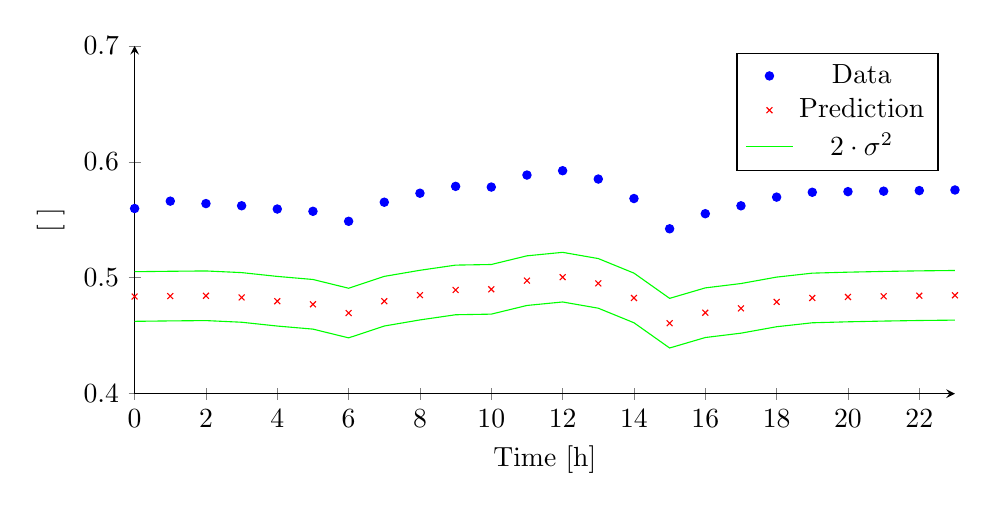
\begin{tikzpicture}
	\begin{axis}[
		xlabel={Time [h]},
		ylabel={[ ]},
		height=6cm,
		width=12cm,
		ymin=0.4, ymax=0.7,
		axis x line=bottom,
		axis y line=left,
%		legend style={at={(axis cs:19,0.425)},anchor=north west},
]
	\addplot[only marks, mark size=1.5pt, color=blue, mark=*] plot coordinates {
		(0, 0.5597241521)
		(1, 0.5660564303)
		(2, 0.5639572144)
		(3, 0.5620805621)
		(4, 0.5592674613)
		(5, 0.5572958589)
		(6, 0.5486843586)
		(7, 0.5651287436)
		(8, 0.5728937387)
		(9, 0.5788049102)
		(10, 0.5781984925)
		(11, 0.5885609388)
		(12, 0.5922956467)
		(13, 0.5851078033)
		(14, 0.5683196783)
		(15, 0.5422233939)
		(16, 0.5552344918)
		(17, 0.5620396733)
		(18, 0.569514811)
		(19, 0.5737179518)
		(20, 0.5742648244)
		(21, 0.5746504068)
		(22, 0.5751609206)
		(23, 0.5756767392)
	};
	\addlegendentry{Data}
	\addplot[only marks, mark size=1.5pt, color=red, mark=x] plot coordinates {
		(0, 0.4838220372)
		(1, 0.4841893317)
		(2, 0.4844607928)
		(3, 0.4830384295)
		(4, 0.4797520441)
		(5, 0.477109649)
		(6, 0.4695569721)
		(7, 0.4797753741)
		(8, 0.485036832)
		(9, 0.4894949128)
		(10, 0.4900254531)
		(11, 0.4975057447)
		(12, 0.5005124745)
		(13, 0.4951399726)
		(14, 0.4825826869)
		(15, 0.4608246327)
		(16, 0.4698541412)
		(17, 0.4736113188)
		(18, 0.4791624125)
		(19, 0.482566695)
		(20, 0.4834080441)
		(21, 0.4840438292)
		(22, 0.4845425981)
		(23, 0.4848678256)
	};
	\addlegendentry{Prediction}
	\addplot[color=green] plot coordinates {
		(0, 0.5052220372)
		(1, 0.5055893317)
		(2, 0.5058607928)
		(3, 0.5044384295)
		(4, 0.5011520441)
		(5, 0.498509649)
		(6, 0.4909569721)
		(7, 0.5011753741)
		(8, 0.506436832)
		(9, 0.5108949128)
		(10, 0.5114254531)
		(11, 0.5189057447)
		(12, 0.5219124745)
		(13, 0.5165399726)
		(14, 0.5039826869)
		(15, 0.4822246327)
		(16, 0.4912541412)
		(17, 0.4950113188)
		(18, 0.5005624125)
		(19, 0.503966695)
		(20, 0.5048080441)
		(21, 0.5054438292)
		(22, 0.5059425981)
		(23, 0.5062678256)
	};
	\addlegendentry{$2\cdot\sigma^2$}
	\addplot[color=green] plot coordinates {
		(0, 0.4624220372)
		(1, 0.4627893317)
		(2, 0.4630607928)
		(3, 0.4616384295)
		(4, 0.4583520441)
		(5, 0.455709649)
		(6, 0.4481569721)
		(7, 0.4583753741)
		(8, 0.463636832)
		(9, 0.4680949128)
		(10, 0.4686254531)
		(11, 0.4761057447)
		(12, 0.4791124745)
		(13, 0.4737399726)
		(14, 0.4611826869)
		(15, 0.4394246327)
		(16, 0.4484541412)
		(17, 0.4522113188)
		(18, 0.4577624125)
		(19, 0.461166695)
		(20, 0.4620080441)
		(21, 0.4626438292)
		(22, 0.4631425981)
		(23, 0.4634678256)
	};
	\end{axis}
\end{tikzpicture}

		\caption{Example prediction with uncertainty for the reaction wheel B during September 2008 when increased friction occurred.}
		\label{f:rwb_prediction_example}
		\end{figure}
			
		\paragraph*{Wheel C} \hfill
		
		The prediction for the third wheel again didn't work very well. The model was able to perform well on the training data, but didn't succeed on the the test data ($\varepsilon = 0.0289$ with $\sigma = 0.062$). But this was also expected as the wheel started to show anomalies in 2010 and was multiple times re-lubricated, which might explain the anomalous, non learn-able behaviour.
		
		Here we tried to improve the performance by changing the models size. But neither a reduction nor increase of nodes by a factor of 2 made any improvements. \newline
		Another option was to disable certain input parameters/features in case they had counter-productive effect on the learning. But this again didn't bring any success.
			
		\paragraph*{Wheel D} \hfill
		
		The fourth and last wheel was an interesting case. With all features activated, the performance was quite poor. But just removing the additional friction coefficient feature (not friction torque, which we are predicting) did help to perform better than the baseline ($\varepsilon = 0.0178$ with $\sigma = 0.074$). \newline
		In figure \ref{f:rwd_prediction_example} an example of the prediction with uncertainty with future unseen test data is shown. We can see that the prediction follows the true data as it is able to deduce a good prediction about the friction mostly through the given wheel speed as future input.
		
		\begin{figure}[htb]
		\centering
		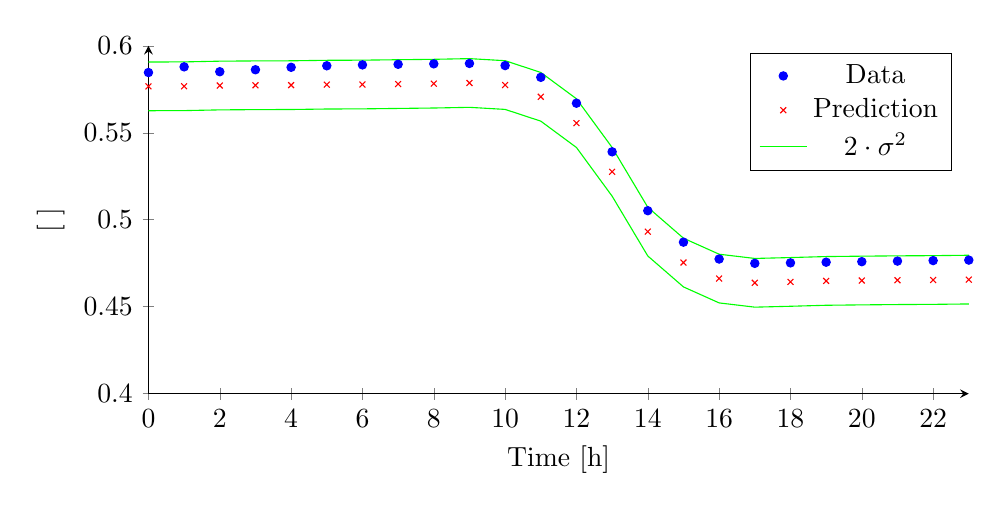
\begin{tikzpicture}
	\begin{axis}[
		xlabel={Time [h]},
		ylabel={[ ]},
		height=6cm,
		width=12cm,
		ymin=0.4, ymax=0.6,
		axis x line=bottom,
		axis y line=left,
]
	\addplot[only marks, mark size=1.5pt, color=blue, mark=*] plot coordinates {
		(0, 0.5846440196)
		(1, 0.5879111886)
		(2, 0.5851085186)
		(3, 0.5862501264)
		(4, 0.5876534581)
		(5, 0.5885193348)
		(6, 0.5890411735)
		(7, 0.5893791318)
		(8, 0.589639008)
		(9, 0.5898739696)
		(10, 0.5886417031)
		(11, 0.5818823576)
		(12, 0.5670129061)
		(13, 0.5390694141)
		(14, 0.5052142143)
		(15, 0.4871221185)
		(16, 0.477432102)
		(17, 0.4749464095)
		(18, 0.4752262831)
		(19, 0.4756105244)
		(20, 0.4759189188)
		(21, 0.4762377143)
		(22, 0.4765394032)
		(23, 0.4768138826)
	};
	\addlegendentry{Data}
	\addplot[only marks, mark size=1.5pt, color=red, mark=x] plot coordinates {
		(0, 0.5766858234)
		(1, 0.5767528488)
		(2, 0.5771701525)
		(3, 0.5773177685)
		(4, 0.577386112)
		(5, 0.5776671827)
		(6, 0.5777555386)
		(7, 0.5779996989)
		(8, 0.5782410524)
		(9, 0.5786328957)
		(10, 0.5774423028)
		(11, 0.5706888248)
		(12, 0.5555401882)
		(13, 0.5275561155)
		(14, 0.4931818014)
		(15, 0.4753986834)
		(16, 0.4662007068)
		(17, 0.4637618943)
		(18, 0.4642703666)
		(19, 0.4648491296)
		(20, 0.4650706633)
		(21, 0.4652549777)
		(22, 0.4653713618)
		(23, 0.4655992947)
	};
	\addlegendentry{Prediction}
	\addplot[color=green] plot coordinates {
		(0, 0.5906858234)
		(1, 0.5907528488)
		(2, 0.5911701525)
		(3, 0.5913177685)
		(4, 0.591386112)
		(5, 0.5916671827)
		(6, 0.5917555386)
		(7, 0.5919996989)
		(8, 0.5922410524)
		(9, 0.5926328957)
		(10, 0.5914423028)
		(11, 0.5846888248)
		(12, 0.5695401882)
		(13, 0.5415561155)
		(14, 0.5071818014)
		(15, 0.4893986834)
		(16, 0.4802007068)
		(17, 0.4777618943)
		(18, 0.4782703666)
		(19, 0.4788491296)
		(20, 0.4790706633)
		(21, 0.4792549777)
		(22, 0.4793713618)
		(23, 0.4795992947)
	};
	\addlegendentry{$2\cdot\sigma^2$}
	\addplot[color=green] plot coordinates {
		(0, 0.5626858234)
		(1, 0.5627528488)
		(2, 0.5631701525)
		(3, 0.5633177685)
		(4, 0.563386112)
		(5, 0.5636671827)
		(6, 0.5637555386)
		(7, 0.5639996989)
		(8, 0.5642410524)
		(9, 0.5646328957)
		(10, 0.5634423028)
		(11, 0.5566888248)
		(12, 0.5415401882)
		(13, 0.5135561155)
		(14, 0.4791818014)
		(15, 0.4613986834)
		(16, 0.4522007068)
		(17, 0.4497618943)
		(18, 0.4502703666)
		(19, 0.4508491296)
		(20, 0.4510706633)
		(21, 0.4512549777)
		(22, 0.4513713618)
		(23, 0.4515992947)
	};
	\end{axis}
\end{tikzpicture}

		\caption{Example prediction with uncertainty of the reaction wheel D. The prediction fits the true data quite well if the standard-deviation is taken into account too.}
		\label{f:rwd_prediction_example}
		\end{figure}
			
		\begin{table}[htb]
		\centering
		\caption{\ac{nn} absolute results and in comparison with the baseline.}
		\begin{tabular}{b{0.25\textwidth}b{0.15\textwidth}b{0.15\textwidth}b{0.15\textwidth}b{0.15\textwidth}}
		\toprule
		Dataset				& $| \varepsilon_{NN} |$	& $\sigma$ 	& Baseline $\Delta\varepsilon$	& $\left| \frac{\varepsilon_{Base}}{\varepsilon_{NN}} \right| - 1$	\\ \midrule
		Wheel A Friction		& $\num{0.0117}$		& $\num{0.0090}$	& $\num{0.0116}$	& 	$\num{99}$\%	\\
		Wheel B Friction		& $\num{0.0321}$		& $\num{0.0107}$	& $\num{-0.0079}$	& $\num{-25}$\%	\\
		Wheel C Friction		& $\num{0.0289}$		& $\num{0.0062}$	& $\num{-0.0023}$	& $\num{-8}$\%	\\
		Wheel D Friction		& $\num{0.0178}$		& $\num{0.0074}$	& $\num{0.0122}$		& $\num{69}$\%	\\
		\bottomrule
		\end{tabular}
		\label{t:rwa_error}
		\end{table}		
			
		\subsubsection{Solar Array}
		The second housekeeping dataset is the solar array, which is taken as one unique unit and therefore only has one prediction. \newline
		As features we have the sunlight incident angle on the array and the voltage as well as the current of the \ac{cm}. Here we also want to predict the next 24 hours.  In the chapter before we have seen, that the voltage is constantly decreasing over time (see figure \ref{f:solar_example}). We started again with our standard model and with all features activated and with an unfortunate poor performance of $\varepsilon = 0.0351$ with $\sigma = 0.0071$, which is factor of 5 above the baseline. The first attempt to improve the performance was made by smoothing the dataset to attenuate the noise level and make it easier to generalize. This gave a slight improvement to the model, but also again to the baseline, leaving the same relative performance gap. \newline
		Therefore the smoothing was undone and the second attempt to improve the network was made. This time the model size was changed with an increase as well as a decreased, which both didn't show any improvements. As last resort the model was reduced to only one dense layer and one feature, resembling a polynomial fit. For the first time, the performance could be improved to $\varepsilon = 0.0100$ with $\sigma = 0.0081$, which is an increase of a factor 3, but still below the baseline.
		
		The example of the solar array shows, that \acp{nn} are no magic bullets for analysing, prediction or extrapolating satellite housekeeping data.